\documentclass{article}
\usepackage[utf8]{inputenc}
\usepackage{graphicx}
\usepackage{amsmath}
\usepackage{caption}
\usepackage{subcaption}
\usepackage[table]{xcolor}


\definecolor{Gray}{gray}{0.9}
\title{Micromechanical Modeling of Dual Phase steel}
\author{Antonia Ramböl Bryntesson}
\date{January 2019}

\begin{document}

\maketitle
\tableofcontents
\section{Introduction}
\section{Materials mechanics}
\subsection{The tensile test}
\label{Section:Tensiletest}
One basic approach to determine the mechanical properties of a material is to perform a tensile test. A specimen of standardized geometry is loaded until fracture. The strain rate is pre-set while the load and elongation is traced. With the data, the force-displacement curve is obtained and this may be transformed to a stress-strain curve.

The first, straight part of the curve, is the linear elastic part. The slope of the curve gives the value of the elastic stiffness, for isotropic materials, Youngs modulus. As the slope of the curve changes, the elastic limit is reached and upon unloading, the deformation is no longer recoverable, a permanent strain is obtained. This limit corresponds to the yield stress. The maximum stress, at the top of the curve, is the ultimate tensile strength. At this point the plastic flow goes from uniform to non-uniform. This is visualised in the specimen as necking. Finally the specimen breaks and the total elongation to fracture is obtained.

The measures above represents different properties.
\begin{itemize}
    \item The elastic stiffness or Young's modulus measures the stiffness, i.e. resistance to flexing.
    \item The yield stress is a measure of the ability to withstand loading and consequently a measure of strength. 
    \item The ultimate tensile stress in relation to the yield stress correlates to toughness, i.e. the ability to loading without a brittle behaviour.
    \item Total elongation to fracture is a measure of ductility.
\end{itemize}

Source:
Lecture notes Metals engineering
\subsection{Stresses and strains}
 The engineering strain and stress visualized in fig...??? is defined, respectively as:

 \begin{subequations}
    \begin{alignat}{2}
        \varepsilon_{eng}=(L-L_0)/L_0 \\
        \sigma_{eng}=F/A_0
    \end{alignat}
    \label{Eq:EngStressStrain}
\end{subequations}
 
 where $L_0$ and $A_0$ is the initial gauge length and initial cross sectional area respectively.
 
 To convert from engineering strain and stress to true strain and stress the following conversion may be made:
 \begin{subequations}
    \begin{alignat}{2}
        \varepsilon_{true}=ln(\frac{L}{L_0}) \\
        \sigma_{true}=\frac{F}{A}=\frac{\sigma_{eng}(1+\varepsilon_{eng})}{A_0}
    \end{alignat}
    \label{Eq:TrueStressStrain}
\end{subequations}

 The engineering stress and strain are based on a constant cross sectional area and gauge length while the true stress and strain are based on a constant volume. This implies that true stress and strain are more accurate for large deformations. 
 
\subsection{Work hardening}
Metallic materials harden when they are subjected to plastic deformation. The yield stress increases with plastic straining. When stresses are exerted crystals slip against each other, which first decrease the strength of the material, but due to the complexity of the crystal structure these slips tend to work as obstacles of further slips and hence increase the strength. The work-hardening is taken into account in the yield criterion as:
\begin{equation}
    f=\varphi(\sigma_{ij})-(\sigma_0 + R)=0
\end{equation}
where $\sigma_0$ is the initial yield stress and $R$ is the hardening variable \cite{Hopperstad}.

The ability to deform plastic depends on the degree to which dislocations are able to move within the material. This will be further discussed in subsequent sections. 

\subsection{Stress Triaxility}
\subsection{Bauschinger effect}



The Bauschinger effect is usually defined as the phenomena where the flow stress of plastic deformation is lower in the reverse direction than in the forward direction. In metals the Bauschinger effect is mainly explained by two mechanisms. The first being long ranged stresses that may be present and helps moving dislocations in the reverse direction. Pile-up of dislocations at the grain boundaries is one such source of long range stresses. The second mechanism is short range effects that cause the resistance of dislocation movement to be less in the original direction than the reverse direction. 

A typical stress strain curve that is obtained when Bauschinger effect is present is shown in fig. \ref{fig:Bauschinger}. The initial yield stress of a ductile material in tension is point A. If the same material was to be exposed to compression instead the yield point would be point E, with approximately the same magnitude. A new specimen is now considered, which is loaded in tension, past the tensile yield strength to point B. The specimen is now unloaded, following the line BC. If a compressive load then is applied plastic flow will start already at point D, which is perceptibly lower than point E, which was the yield strength of the specimen only tested under compression. The yield strength in tension was increased from A to B by strain hardening, while the yield strength in compression was decreased. This is the Bauschinger effect. 

If the material is loaded such that the loop is closed, a mechanical hysteresis loop is obtained.

\begin{figure}[h!]
    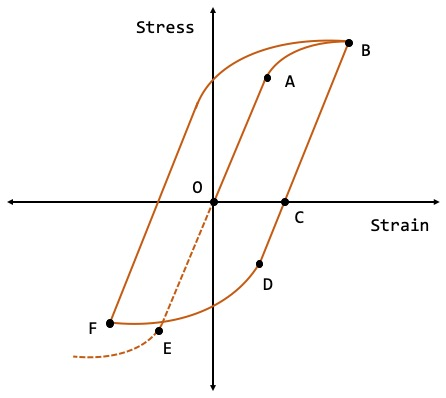
\includegraphics[width=\linewidth]{Bauschinger.jpg}
    \caption{Bauschinger effect and hysteresis loop}
    \label{fig:Bauschinger}
\end{figure}

The magnitude of the Bauschinger effect has been found to be rather small in pure metals but profoundly larger in alloys with hard, non-shearable second phases. 

\subsection{Ductile fracture} \label{Section:DuctileFracture}

Nucleation, growth and coalescence of microscopic voids that initiates at impurity atoms and second phase particles is usually the reason why ductile materials fail. Pure materials with a very small volume fraction of inclusions may have a very large elongation to fracture, while high impurity metals fracture at a much lower strain, as illustrated in fig.(\ref{fig:TensileDeformation}). The reason is that voids nucleate at inclusions and second-phase particles. These voids then coalescence and a microcrack is formed, which lead to loss of load bearing capacity and fracture.

\begin{figure}[h!]
    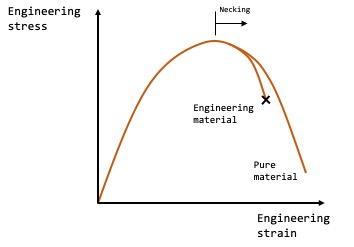
\includegraphics[width=\linewidth]{TensileDeformation.jpg}
    \caption{A crystal lattice of periodic unit cells}
    \label{fig:TensileDeformation}

\end{figure}

Usually the process of ductile fracture can be divided into three stages:

\begin{enumerate}
\item A free surface starts to form at a second-phase particle or inclusion by either interface decohesion or cracking of the particle. 
\item The void grows around the particle as a consequence of plastic strain and hydrostatic stress.
\item The growing void coalescence with neighbouring voids.
\end{enumerate}

For a void to form around a particle a sufficiently large stress is needed to break the interfacial bonds between the particle and the matrix. There exist numerously of models to estimate the void nucleation stress. The most commonly used model by \cite{Argon} is based on that the interfacial stress at a cylindrical particle is approximately equal to the sum of the mean hydrostatic stress and the effective von Mises stress. The sum of these two stresses defines the decohesion stress. According to this model, the nucleation strain decreases as the hydrostatic stress increases. This means that void nucleation occurs more often in a triaxial tensile stress field, which according to \cite{FractureMechanics} is a result that is consistent with experimental observations. 

Once a void has formed, they grow and coalescence as a result of further plastic strain and hydrostatic stress. The process is illustrated in fig. \ref{fig:Voidnucleation}.

\begin{figure}[h!]
    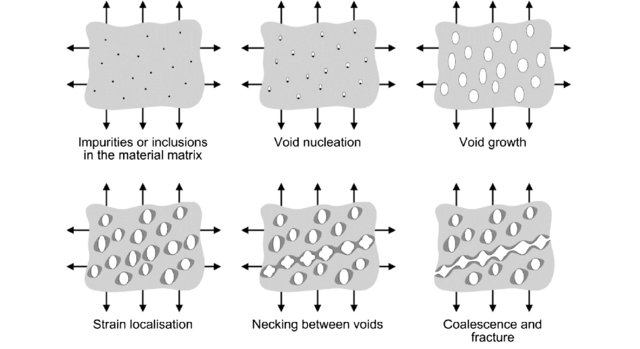
\includegraphics[width=\linewidth]{Voidnucleation.jpg}
    \caption{Void nucleation, growth and coalescence in ductile materials: (a) inclusions in a ductile matrix, (b) void nucleation, (c) void growth, (d) strain localization between voids, (e) necking between voids, (f) void coalescence and fracture \cite{FractureMechanics}.}
    \label{fig:Voidnucleation}

\end{figure}
\subsection{Modeling of Porous plasticity}
When modelling porous metal plasticity the model is usually assumed to consist of a matrix material with a certain fraction of voids. In contrast to metals in general, which are assumed to be pressure-insensitive, porous metals are compressible. During straining both volumetric and deviatoric plastic strains develop. There is a competition between the matrix material which work-hardens and the voids which nucleate and grow and softens the material. 

A popular model for describing porous metal plasticity is one that first was proposed by Gurson and later modified by Tvergaard and Needleman. This model analyzes the plastic flow in a porous medium by assuming that the material is a continuum. The voids are taken into account by their influence on the global flow behaviour. Since the material is assumed to be continuous and homogeneous the effect of the voids is averaged through the material \cite{FractureMechanics}. The yield criterion in this model is defined as

\begin{equation}
  f=\frac{\sigma^2_{eq}}{\sigma^2_M}+2f\beta_1cosh(\frac{\beta_2\sigma_{kk}}{2\sigma_M})-1-\beta_3f^2=0  
 \label{Eq.:GursonYield}
\end{equation}

where $q_1$, $q_2$ and $q_3$ are phenomenological fitting parameters. $q_1$ modifies the void volume fraction and thus affects the yielding, $q_2$ is a correction factor for the hydrostatic stress and $q_3={q_1}^2$. The three parameters together affects the form of the yield surface. Values of $q_1 = 1.5$, $q_2 = 1.0$ and $q_3 = q_1^2$ are typical values for metals. With $f=0$ the von Mises yield surface for an incompressible material is recovered. Further, $\sigma_M$ is the flow stress of the  matrix material and $\sigma_{eq} =\sigma_{VM}$ is the equivalent von Mises stress. $f$ is the void volume fraction. \\

According to \cite{FractureMechanics} voids grow very rapidly when the void fraction exceeds 10 to 20\%. In equation (\ref{Eq.:GursonYield}) the rapid void growth and coalescence of the final stage is not sufficiently captured. Failure is hence often assumed when a critical fraction $f_C$ is reached, where a typical value for carbon steels is $f_C = 0.15$. When the critical value is exceeded there is only a small amount of additional macroscopic strain before failure in real materials, which makes the assumption of failure at $f_C$ reasonable. Tvergaard - Needleman modified the original model by replacing the volume fraction $f$ with an effective void volume fraction $f^*$ which take into account void nucleation and coalescence, in an attempt to capture the final stage before failure. This parameter is defined as:


    

\begin{equation}
    f^*=
    \begin{cases}
        f & \text{if}\    f \leq f_C\\
        f_C+\frac{\overline{f_F}-f_C}{f_F-f_C}(f-f_C) & \text{if}\ f_C\leq f \leq f_F\ \text{where}\ \overline{f_F}=\frac{q_1+\sqrt{q_1^2-q_3}}{q_3}\\
        \overline{f_F} &\text{if}\ \geq f_F 
    \end{cases}
    \label{Eq:FractureCriteria}
\end{equation} 

where $f_C$ is the critical void volume fraction and $f_F$ is the void volume fraction at which there is a complete loss of load bearing capacity. According to \cite{UsersManMetalPlast}, the above form of nucleation has shown accurate results for low triaxiality but is less exact for high triaxiality. 

\section{Metallurgy}
\label{section:Metallurgy}
\subsection{Crystal structure}
Most metals are crystalline materials which means that they have a periodic structure of unit cells, together forming the crystalline lattice. The unit cell is the smallest repetitive structure that, in the case of a metallic crystal structure, will by translation form the atomic or molecular structure. 

\begin{figure}[h!]
    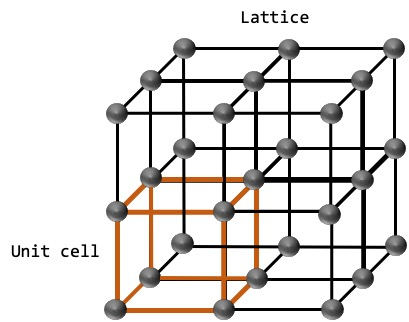
\includegraphics[width=\linewidth]{Unitcell.jpg}
    \caption{A crystal lattice of periodic unit cells}
    \label{fig:Unitcell}

\end{figure}


In total seven crystal structures have been found, in metals three of them are the most common, namely the Body-centered Cubic (BCC), Face-centered Cubic (FCC) and Hexagonal Closed Packed (HCP). In the figure below, also the Body Centred Tetragonal (BCT) structure is presented. This is the structure of martensite.
\begin{figure}[h!]
    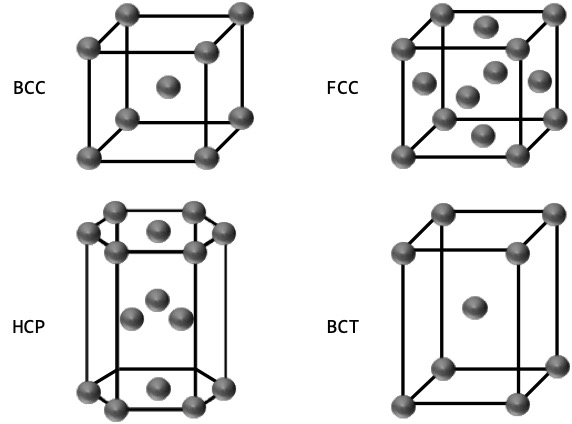
\includegraphics[width=\linewidth]{Crystalstructures.jpg}
    \caption{The three most common crystal structures in metals and the crystal structure of martensite}
    \label{fig:Crystal structures}

\end{figure}

The elastic behaviour is only dependent on the crystal structure. The stretching of the bonds between the atoms is what sets the value of Young's modulus. Hence, the elastic stiffness is independent of microstructural factors such as grain size. Even alloying elements have little effect, as long as they don't change the crystal structure. The temperature, however, affects the equilibrium separation of the atoms (it increases), which the modulus depends on. This leads to that the Young's modulus tends to decrease with increasing temperature.

\subsection{Defects and strengthening mechanisms}
How the material behaves in the plastic domain depends on both the crystal structure and defects in the structure. The mechanical properties of metals are strongly dependent on the defects in the material. A structure containing a defect has a lower state of total energy than a defect-free structure, hence all metals contain defects. The defects can be either point defects, line defects, planar/surface defects or volume defects.  

\subsubsection{Point defects}

Point defects are vacancies, substitutional atoms, self-interstitial atoms and interstitial impurity atoms. Vacancies are voids where an atom is missing. Substitutional atoms are atoms of a different kind than the the bulk material, that have taken the position of a host-atom in the lattice. These atoms are usually close in size to the host-atom. Interstitially impurity atoms take positions in between the host atoms, and are hence usually smaller in size compared to the host atoms. Carbon in steel is one example. Self-interstitial atoms are extra atoms of the bulk material. 

Solid solution strengthening is a strengthening mechanism due to point defects where dislocations interact with foreign atoms that are in solid solution. The strengthening mechanism is due to the associated strain fields that occur around both interstitial and substitutional solute atoms that are in mismatch with the host atoms. The mismatch is regarding differences in size and shear modulus. 

Particle strengthening is yet another strengthening mechanism connected to point defects. When fine particles are dispersed in the lattice they act as obstacles and particle strengthening, or dispersion strengthening is obtained. Particle strengthening can occur as a consequence of two different mechanisms. The first one is due to the so called Orowan mechanism where the dislocations bow around obstacles, or more specific, incoherent particles. With coherent or semi-coherent particles the strengthening mechanism is instead due to shearing of the particles. 

\subsubsection{Line defects}

Line defects are dislocations, areas in the lattice structure that are out of place in the crystal structure. When a stress is applied, dislocations are formed and moved and lead to slips - plastic deformation. There are two types of dislocations, edge - and screw dislocations. 

The edge dislocation can be seen as an extra half-plane in the lattice. The reason why the dislocation is called a line defect is because the locus of the defected points due to the dislocation lie along a line, a line running perpendicular to the extra half plane (illustrated as the dotted black line in the figure). The dislocation allow for deformation to occur at a much lower stress than in a perfect crystal. The reason for the case with edge dislocation is because, small parts can move bit by bit instead of that the whole structure would have to move at once, thus only a few bonds have to break at a time. This require a much smaller force. The dislocation is slipping one plane at a time. Finally, the movement of the dislocation lead to that the upper part of the structure move in relation to the lower part.

\begin{figure}[h!]
    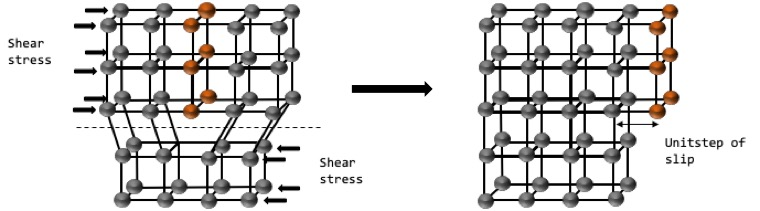
\includegraphics[width=\linewidth]{Edgedisl.jpg}
    \caption{Movement of an edge dislocation}
    \label{fig:Edge dislocation}

\end{figure}

Screw dislocations and their movement is also a consequence of shear stress. The direction of the dislocation motion is perpendicular to the stress direction, in contrast to for the edge dislocation. The process can be visualized as a block of metal being ripped by a shear force acting in different direction in the upper and lower part of the block. Also in this case, only a small portion of bonds have to be broken at a time, which require a smaller force than breaking all the bonds in the middle plane simultaneously. 
\begin{figure}[h!]
    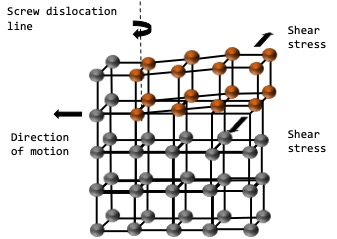
\includegraphics[width=\linewidth]{Screwdis.jpg}
    \caption{Screw dislocation}
    \label{fig:Screw dislocation}

\end{figure}
The stress required to move the dislocation is called the Peierls-Nabarro stress. This stress is higher if the spacing between the atoms is large, hence dislocations move along the densest planes of atoms in the structure. FCC and BCC metals are dense and thus often ductile. In order to strengthen the metals the movement of the dislocations have to be hindered, which can be done by obstacles like point defects, grain boundaries or by plastically deform the metal such that a large number of dislocations are formed and pin each other, strain hardening \cite{Hardening}.



\subsubsection{Planar defects}
Planar defects can be stacking faults, twin boundaries or grain boundaries. 

Stacking fault is when the sequence of the stacking of the planes is interrupted in one or two layers. If the stacking is not corrected immediately but continues a second stacking fault will form, which is a twin of the first one and a twin boundary is obtained. 

Grain boundaries acts as obstacles for the motion and length of the dislocations. 
At the grain boundary there is an increased disorder which causes discontinuity in the slip planes. With decreased grain size, the grain boundary area is increased, hence the material is strengthened. Grain size strengthening not only increase the strength, but also improve the toughness \cite{Metalseng}. The size of the grain boundary strengthening is given by the Hall-Petch relation:
\begin{equation}
    \sigma_y= \sigma_0 + \frac{k_y}{d^\frac{1}{2}}
    \label{Eq:Hall-Petch}
\end{equation}

where $\sigma_0$ represent the yield strength of the single crystal material, $k_y$ is a grain boundary strengthening factor that is material specific and d is the grain diameter. 

\subsubsection{Volume defects}
Volumetric defects acts on a much larger scale than defects mentioned above, but they still affect the movement of the dislocations. Voids are example of volumetric defects and are defined as regions where a large number of atoms are missing. 

Another form of volumetric defect occurs when impurity atoms cluster together and form regions of another phase, which is called precipitates.  

\section{Dual-phase steels}
Dual phase steel is a steel in the Advanced high strength steel (AHSS) family and has been developed since the 1970s. The microstructure of a ferritic phase with dispersed islands of martensite give the material its characteristic combination of properties, low initial yield stress, great ductility due to the soft ferrite, high ultimate tensile strength because of the hard martensite and a high initial strain hardening. These features make the steel an excellent choice of material in the automotive industry. Weight reduction of the car body, increasing passive safety systems and energy savings are benefits that the increased usage of DP-steel has contributed to. 

\begin{figure}[h!]
    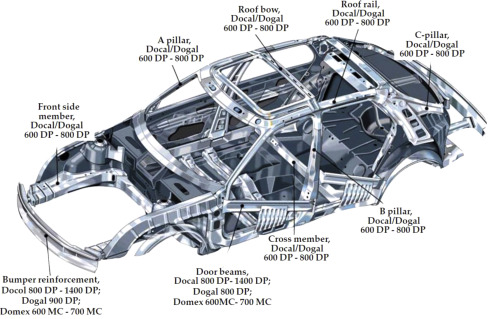
\includegraphics[width=\linewidth]{DPinCars.jpg}
    \caption{Application of DP-steel in cars, \cite{Fonstein}}
    \label{fig:DP in cars}

\end{figure}



\subsection{Microstructure}
The microstructure of martensitic islands embedded in a matrix of ferrite is obtained from an inter critical heat method of an initial phase of ferrite and pealite. The heating is followed by an accelerating cooling. When the temperature during heating reaches $A_1$ austenite appear. It is the austenite that later, during quenching, transform to martensite, thus is the holding time above $A_1$ crucial for the final volume fraction of martensite \cite{Chatterjee}.  

\begin{figure}[h!]
    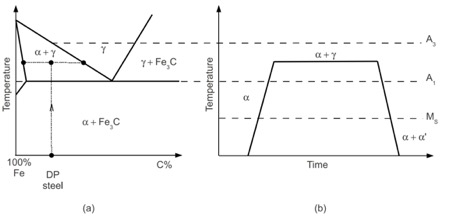
\includegraphics[width=\linewidth]{DPManufacturing.jpg}
    \caption{Heat treatment when manufacturing DP-steel: (a) schematic Fe-C diagram, (b) applied heat treatment, \cite{Landron}}
    \label{fig:Manufacturing}

\end{figure}

Apart from martensite, bainite and retained austenite components may also exist. These are usually produced when improved edge stretch formability is desired.  The ferritic phase is the soft phase providing great ductility and low initial yield strength while the islands of hard martensite give the material high ultimate tensile strength(4). 



\subsection{Influence of alloying elements}
To achieve the required microstructure additions of alloying elements are important. The carbon content is usually 0.06-0.15 wt to give the martensite its strength. Manganese is added to solid solution strengthening ferrite. Both carbon and manganese also stabilize the austenite. To prevent forming of pearlite and bainite, chromium and molybdenum is added and for promoting ferrite transformation silicon is added. Further, vanadium and niobium precipitation strengthen the material and refines the microstructure \cite{BookFlake}. 


\subsection{Influence of carbon}
The carbon content in DP-steels affects both the microstructure and the mechanical properties.  

Depending on the carbon content the martensite will appear in different morphologies, according to \cite{Granbom}. With a low to medium level of carbon content (up to 0.6 wt\%) in the martensite a lath type of martensite is obtained. The type of lath also varies with the carbon content, where a higher carbon content gives a more massive and dense appearance compared to martensite with a lower carbon content. 

The hardness of the martensite is also affected by the carbon content to a great extent, where a higher carbon content gives a harder martensite. As a consequence a high carbon content steel will have different mechanical properties compared to a low carbon content steel. 



\subsection{Influence of grain refinement}
Yield strength and tensile strength increases with grain refinement. That has been stated frequently in the literature, and the study by Calcagnotto is a great example. DP-steels with approximately the same volume fraction of martensite and chemical composition, but with different grain sizes were studied. Conclusions made in the study were, except from that a decrease in grain size lead to increased yield strength and tensile strength also that uniform elongation and total elongation are hardly affected while the initial strain hardening rate increase. The increase in initial strain hardening rate is due to a higher number of dislocation sources, early interactions of the dislocations and the back stresses that are due to both martensite islands and ferrite grains smaller than 1 $\mu m^3$. Further more it was stated that an increase in yield strength and the strain hardening rate of the ferrite matrix due to grain refinement results in rapid stress transfer to martensite. The consequence being that the yield stress of the martensite is reached at lower strains than in microstructures with coarser grains. 

\subsection{Influence of volume fraction and distribution of phases}
The transformation of austenite to martensite is associated with a volume expansion with strains being produced. These strains results in residual stresses in the ferrite surrounding the martensite islands. According to [19 ] the internal stresses are assumed to promote plastic flow, thus lowering the point of yielding. Yet another consequence of the volume expansion is that plastic deformation is induced in neighbouring ferrite grains and a larger number of unpinned dislocations are produced nearby martensitic grains. These dislocations are assumed to be free to move early in the deformation process, hence contributing to the strain hardening. 

With a higher fraction of martensite, more residual stresses are produced. Hence the steel yield at lower strains and the initial strain hardening is higher, compared to with lower volume fractions of the hard phase. 

\section{Microstructure based model}
\label{Micromodel}
A model proposed by \cite{Gutierrez} and frequently used by \cite{Ramazani} for describing the material behaviour of the DP-steel is used in this work. Each phase is modelled separately but are based on the same theory and equations. The model and the resulting flow curves emerges from the dislocation theory and the magnitude of strain hardening is based on dislocation density. In this work the Hall-Petch grain boundary strengthening is added to the model. The elastic modulus for both phases is assumed to be 210 GPa. The flow stress consists of two parts, one strain independent friction stress and one strain dependent hardening stress as:

\begin{equation}
   \sigma = \sigma_{friction} + \sigma_h = \sigma_0 + \Delta\sigma + \sigma_d + \sigma_h
   \label{Eq:Flowstress}
\end{equation}

where 

\begin{itemize}
    \item $\sigma_0$ - the combined contribution from the Peierls stress and the strengthening from solute atoms
        \begin{equation}
        \label{PeierlsStress}
        \begin{split}
          \sigma_0 &= 77+750(\%P) + 60(\%Si) + 80(\%Cu) + 45(\%Ni) + 60(\%Cr)\\
                & + 80(\%Mn) + 11(\%Mo) + 50(\%N_{ss})
          \end{split}
        \end{equation}
  
    \item $\Delta\sigma$ - the strengthening from C in solid solution and precipitates\\
    
            For ferrite:
            
            \begin{equation}
            \label{solidsolM}
                 \Delta\sigma=5000(\%C_{ss}^f)  
            \end{equation}
    
    
    
        For martensite:
        \begin{equation}
        \label{solidsolM}
            \Delta\sigma=3065(\%C_{ss}^m)-161
        \end{equation}
    
    

    \item $\sigma_d$ - Hall- Petch strengthening. Accounts for grain boundary strengthening.
    
    \begin{equation}
        \sigma_d = \frac{K}{\sqrt{d}}
    \end{equation}
    
    \item $\sigma_h$ - the work hardening due to dislocation accumulation, defined by the Taylor equation\\
    
    The work hardening R($\rho$) is defined from dislocation mechanics through the Taylor equation:
    
    \begin{equation}
    \label{Eq:Tayloreq}
        R(\rho)=\alpha M \mu b \sqrt{\rho}
    \end{equation}
    
Where M is the Taylor factor, b is the Burgers vector, $\alpha$ is a constant and $\rho$ is the dislocation density.    

   
The evolution of dislocation density with strain during deformation can be split into a dislocation storage term and a dislocation annihilation term as:

\begin{equation}
\label{Eq:DislocationSplit}
    \frac{d\rho}{d\gamma}=\frac{d\rho}{d\gamma}_{stored} + \frac{d\rho}{d\gamma}_{annihilation}
\end{equation}

The change in dislocation density as a function of the macroscopic equivalent strain is obtained by substituting $d\gamma=Md\epsilon$ in equation \ref{Eq:DislocationSplit}. 

\begin{equation}
    \frac{d\rho}{d\gamma}=M (\frac{1}{bL}-k_r\rho)
\end{equation}

Integration of the evolution equation for dislocation density:

\begin{equation}
    \int_{\rho_0}^{\rho} \frac{d\rho}{\frac{1}{bL}-k_r\rho} = \int_{0}^{\epsilon^p} Md\epsilon^p
\end{equation}

Where $\rho_0$ is the initial dislocation density in the undeformed material and L is the dislocation mean free path, which in the integration is assumed constant and $k_r$ is a parameter controlling dynamic recovery rate. With the result from the integration substituted into equation \ref{Eq:Tayloreq} the contribution from work hardening is expressed as:

\begin{equation}
    R(\epsilon^p) = \alpha M \mu \sqrt{b} \sqrt{\frac{1}{b L k_r}[1-exp(-k_r M\epsilon)]+\rho_p exp(-k_r M\epsilon)}
\end{equation}

Since the initial dislocation density usually is relatively low, $\rho_0$ may be neglected, giving the resulting equation:

    \begin{equation}
        \sigma_h=\alpha M \mu \sqrt{b} \sqrt{\frac{1-exp(-M_T k_r \varepsilon)}{k_r L}} 
    \end{equation}

Where $\varepsilon$ is the plastic strain. According to \cite{Ramazani} the following values of the constants may be used.
$\alpha=1/3$, 
$M_T=3$, 
$\mu=80$ GPa, 
$b=2.5*10^{-10}$, 

$k_r$  for ferrite = $\frac{10^{-5}}{d_f}$ where $d_f$ is the grain size of ferrite and for martensite = 41. 
$L$ for ferrite =$d_f$ m and for martensite  =$3.8\times10^{-8}$ m is used.  
\end{itemize}    

Some parameters are though rather case specific and should be fitted to experimental data. These include the Hall-Petch constant for both ferrite and martensite ($K_d$ and $K_m$), the constant and the factor in equation \ref{solidsolM} and the parameter controlling dynamic recovery rate ($k_r$). 

\section{The axisymetric model}
\label{Section:Axisym}
The DP-steel with its distinguishable two phases, can be accounted for as a heterogeneous material at the micro level. Numerously researches, e.g. \cite{Ramazani} and \cite{Uthaisangsuk},  have shown that micromechanical modeling using numerical tensile test of a representative volume element, in order to study the flow stress and also damage of multiphase steels, is a well suited approach. 

The numerical simulation of the plastic flow behaviour of the DP steel is presented by unit cells consisting of a solid sphere embedded in a cylinder, where the sphere represents the martensite and the cylinder the ferrite. The cylinders are axisymmetric cells and are approximations of a hexagonal cylinders that are periodically stacked on the macroscopic scale, which is illustrated in fig. \ref{fig:PeriodicaRVE}. This model is based on the one described by \cite{Lai}. 

\begin{figure}[h!]
    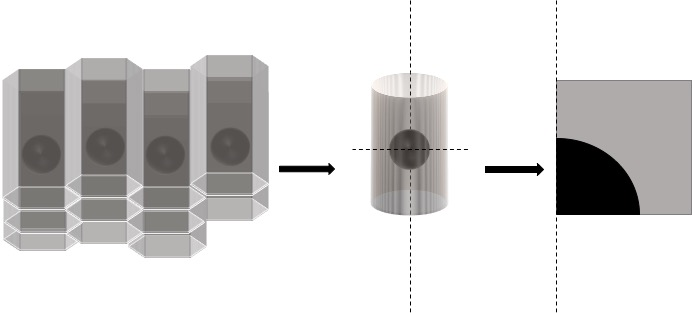
\includegraphics[width=\linewidth]{PeriodicRVE.jpg}
    \caption{}
    \label{fig:PeriodicaRVE}

\end{figure}

This particular model, as a choice of RVE, has been reported by eg. \cite{Al-Abbasi2003} and \cite{Lai}, to give successful results when simulating DP-steel. The reason for the good results despite the simplicity of the model is, according to \cite{Lai} probably due to that the model manage to capture the main factors governing the behaviour of the steel under uniaxial tension, namely the volume fraction of the two phases, the constitutive response of respective phase and how they interact. 

To obtain the desired volume fraction martensite $Vf_m$ the radius of the martensitic sphere is calculated as:
\begin{subequations}
    \begin{alignat}{4}
        V_sphere=\frac{4\pi r^3}{3} \\
        V_cylinder= 2\pi s^2 h\\
        V_sphere/V_cylinder = \frac{2r^3}{3h^2}\\
        r=(\frac{3 V_m h^3}{2})^{1/3}
    \end{alignat}
    \label{Eq:CalcVol}
\end{subequations}



\begin{figure}[h!]
    \centering
    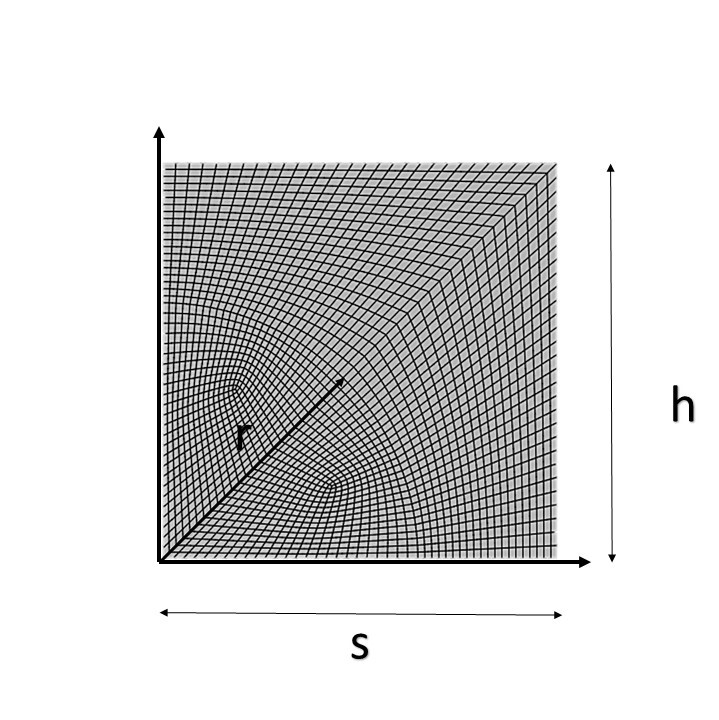
\includegraphics[width=0.8\linewidth]{Axisymmodel.jpg}
    \caption{Geometry for calculating desired volume fraction of respective phase}
    \label{fig:my_label}
\end{figure}

\subsection{Periodic boundary condition}
In order for the simulation of a tensile test on a unit cell to represent the macroscopic response, periodicity in the boundary conditions is crucial. This to maintain connectivity throughout the deformation process. In this case, with a cylinder as the unit cell, the outer surface has to be kept vertical, and for the axisymmetric model, to keep edge E3 vertical. This is ensured by applying constraints. One way of describing the periodic constraints is given by \cite{Lai}:


\begin{subequations}
    \begin{alignat}{4}
        u_3(r,z=h)=\overline{u_3}, \quad 0 < r <s \label{Eq:loading}\\
        u_3(r,z=0)=0, \quad 0 < r <s \label{Eq:sym1}\\
        u_1(r=0,z)=0, \quad 0 < z <h \label{Eq:sym2}\\
        u_1(r=s,z)=\overline{u_1}, \quad 0 < z <h \label{Eq:Horisdisp}
    \end{alignat}
\end{subequations}

In condition \ref{Eq:loading} a uniform displacement is applied, which corresponds to the macroscopic strain during the tensile test. Displacement $\overline{u_1}$ in \ref{Eq:Horisdisp} is unknown, but also uniform in order to maintain periodicity. Condition \ref{Eq:sym1} and \ref{Eq:sym2} ensure symmetri with respect to the rotation axis E1 and the side E2.

The axisymmetric model and the uniaxial tension test is simulated by the finite element method using ABAQUS. The chosen elements are quadrangular with second-order interpolation function.  For DP500, DP600 and DP800 reduced integration is used (CAX8R) while for DP980 full integration (CAX8) is needed to avoid distortion. The initial meshes have about 3000 elements, mesh sensitivity is studied in section \ref{SensStudyMesh}. Abaqus Implicit is used for the models that only simulate plastic deformation, while when ductile metal plasticity with a fracture criteria is added to the simulation, Abaqus Explicit is required. 

\section{Experimental procedures and results}
The four DP-steels, DP500, DP600, DP800 and DP980, delivered by SSAB was characterized and tested in microstructural- and mechanical properties. For mec
\subsection{Microstructure characterization}
The microstructure of the four DP-steel, DP500, DP600, DP800 and DP980 is characterized by studying EBSD (Electron Backscatter Diffraction). Three separate areas of 80 $\mu m \times 80 \mu m$ was studied for each steel. To identify martensite IQ maps were used and for the distribution and size of martensite islands, binary maps were studied.

For calculating linear size of martensite and free path of ferrite the following equations were used:

\begin{subequations}
    \begin{alignat}{2}
        L_d=2\times \frac{V_d}{P_L} \\
        L_m=2\times \frac{V_m}{P_L}
    \end{alignat}
    \label{Eq:LinSize}
\end{subequations}
 
 $P_L$ is the number of intersections per $\mu m$ on 80 horizontal lines and 80 vertical lines in the skeleton images shown in fig. \ref{fig:Micro2_500}, \ref{fig:Micro2_600}, \ref{fig:Micro2_800} and \ref{fig:Micro4_500}.
 
 For identifying ferrite grain size an area was first calulated by counting number of points inside a grain. The diameter of the grain was the obtained by assuming the grain to be circular and then the diameter of the circle. The ferrite grain maps are shown in fig. \ref{fig:Micro3_500}, \ref{fig:Micro3_600}, \ref{fig:Micro3_800} and \ref{fig:Micro3_500}.
 
 All microstructure data is given in table \ref{tab:MicrostructurePara}


\begin{figure}[h!]
     \centering
     \begin{subfigure}[b]{0.3\textwidth}
         \centering
         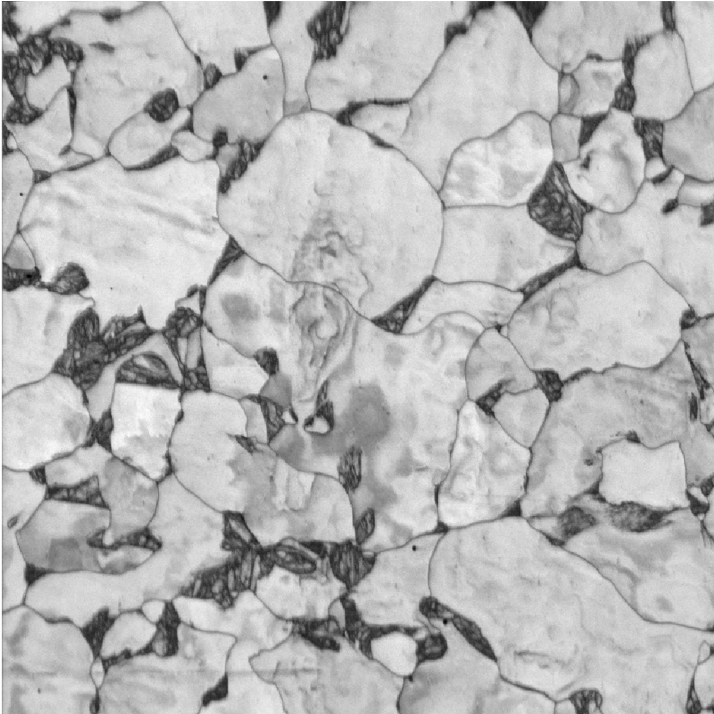
\includegraphics[width=\textwidth]{Micro1_500.png}
         \caption{}
         \label{fig:Micro1_500}
     \end{subfigure}
     \hfill
     \begin{subfigure}[b]{0.3\textwidth}
         \centering
         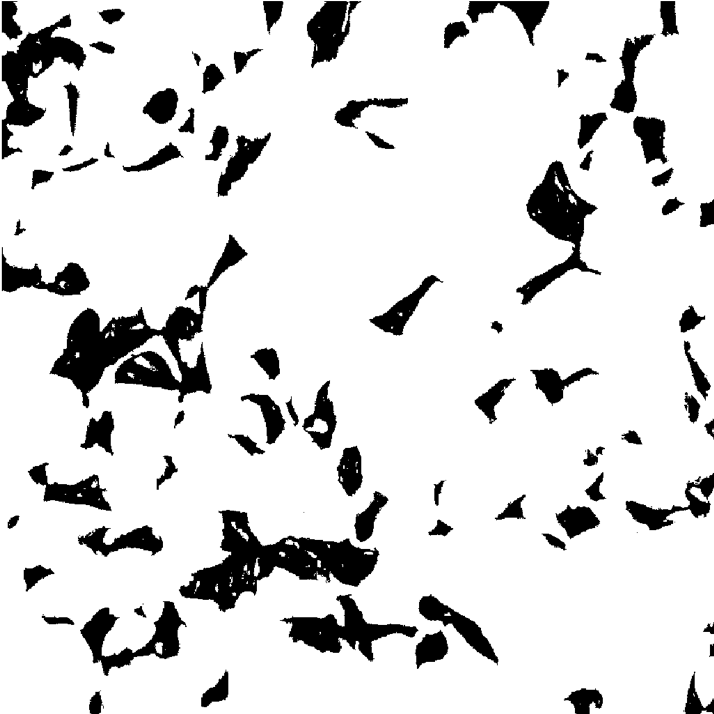
\includegraphics[width=\textwidth]{Micro2_500.png}
         \caption{}
         \label{fig:Micro2_500}
     \end{subfigure}
          \hfill
     \begin{subfigure}[b]{0.3\textwidth}
         \centering
         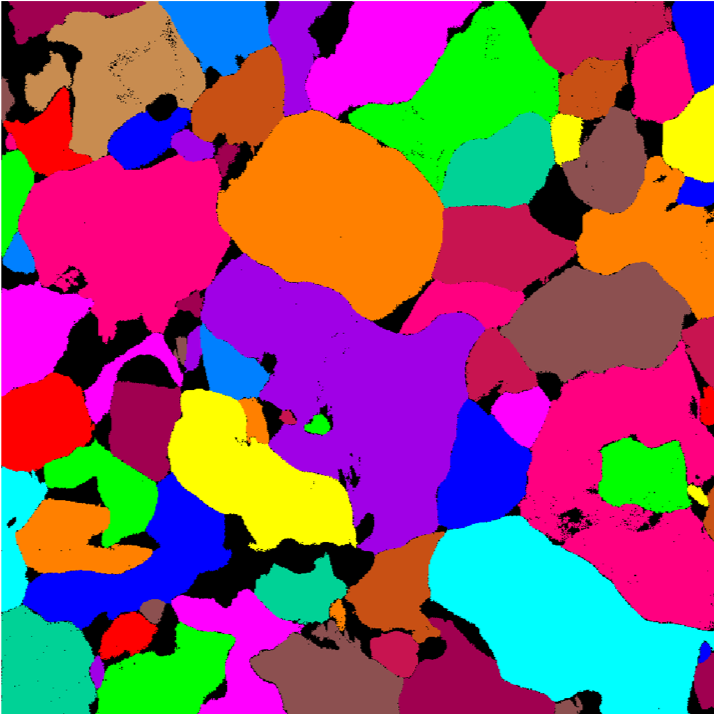
\includegraphics[width=\textwidth]{Micro3_500.png}
         \caption{}
         \label{fig:Micro3_500}
     \end{subfigure}
     \caption{Microstructure of DP500}
     \label{fig:Micro_500}
\end{figure}

\begin{figure}[h!]
     \centering
     \begin{subfigure}[b]{0.3\textwidth}
         \centering
         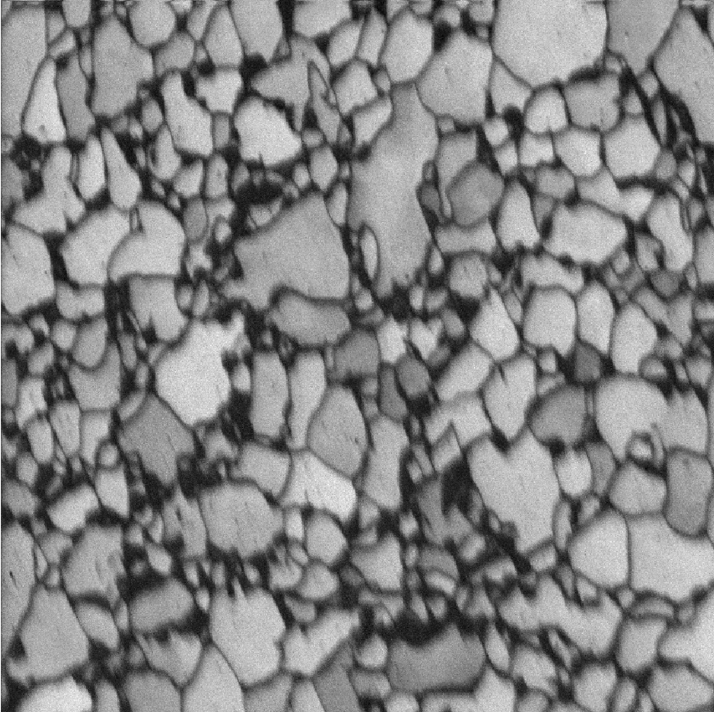
\includegraphics[width=\textwidth]{Micro1_600.png}
         \caption{}
         \label{fig:Micro1_600}
     \end{subfigure}
     \hfill
     \begin{subfigure}[b]{0.3\textwidth}
         \centering
         
\includegraphics[width=\textwidth]{Micro2_600.png}
         \caption{}
         \label{fig:Micro2_600}
     \end{subfigure}
          \hfill
     \begin{subfigure}[b]{0.3\textwidth}
         \centering
         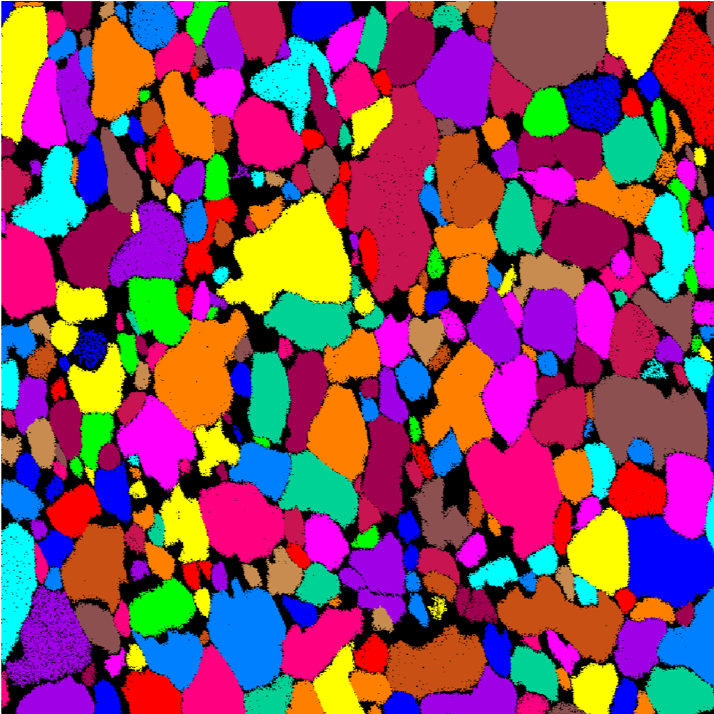
\includegraphics[width=\textwidth]{Micro3_600.png}
         \caption{}
         \label{fig:Micro3_600}
     \end{subfigure}
     \caption{Microstructure of DP600}
     \label{fig:Micro_600}
\end{figure}

\begin{figure}[h!]
     \centering
     \begin{subfigure}[b]{0.3\textwidth}
         \centering
         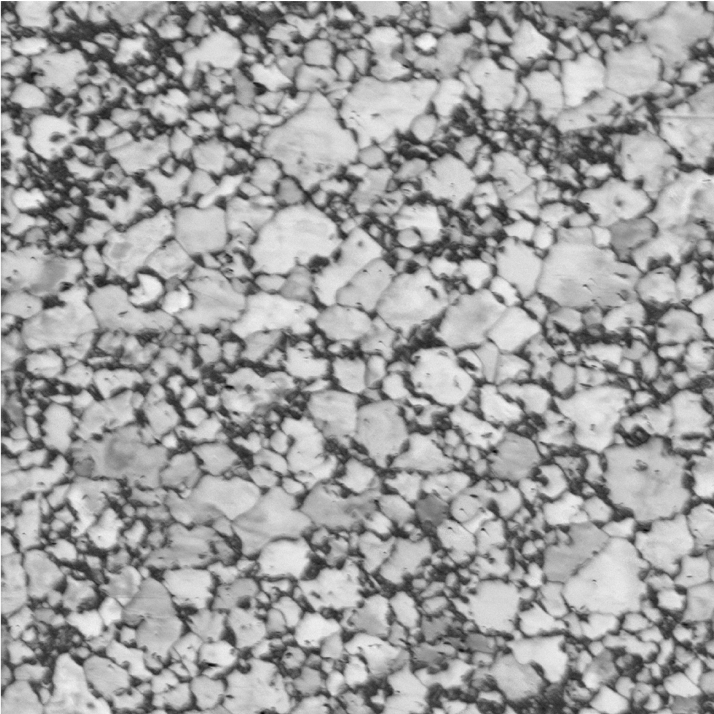
\includegraphics[width=\textwidth]{Micro1_800.png}
         \caption{}
         \label{fig:Micro1_800}
     \end{subfigure}
     \hfill
     \begin{subfigure}[b]{0.3\textwidth}
         \centering
         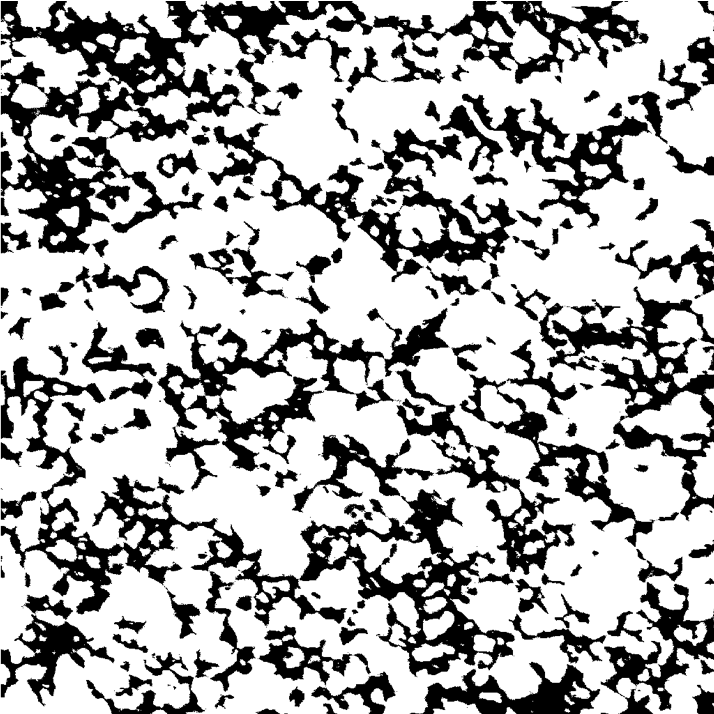
\includegraphics[width=\textwidth]{Micro2_800.png}
         \caption{}
         \label{fig:Micro2_800}
     \end{subfigure}
          \hfill
     \begin{subfigure}[b]{0.3\textwidth}
         \centering
         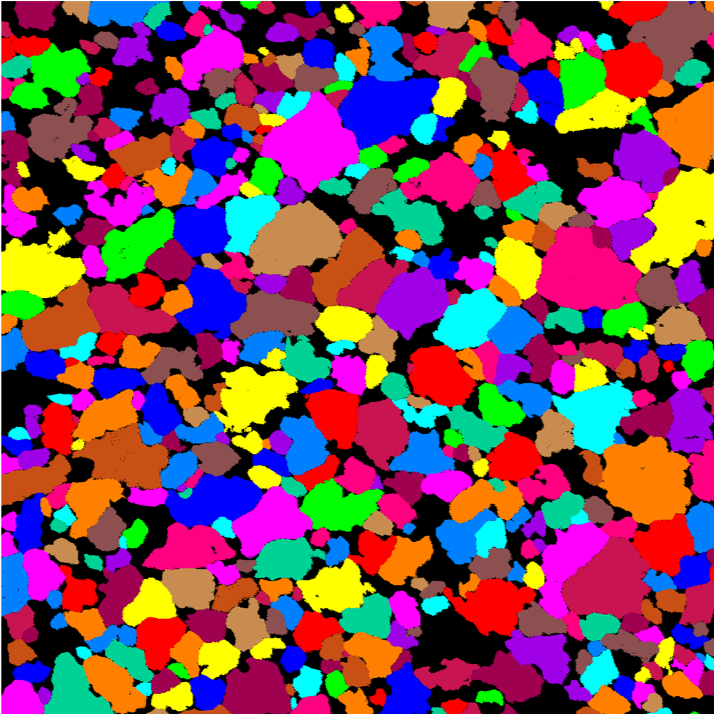
\includegraphics[width=\textwidth]{Micro3_800.png}
         \caption{}
         \label{fig:Micro3_800}
     \end{subfigure}
     \caption{Microstructure of DP800}
     \label{fig:Micro_800}
\end{figure}

\begin{figure}[h!]
     \centering
     \begin{subfigure}[b]{0.3\textwidth}
         \centering
         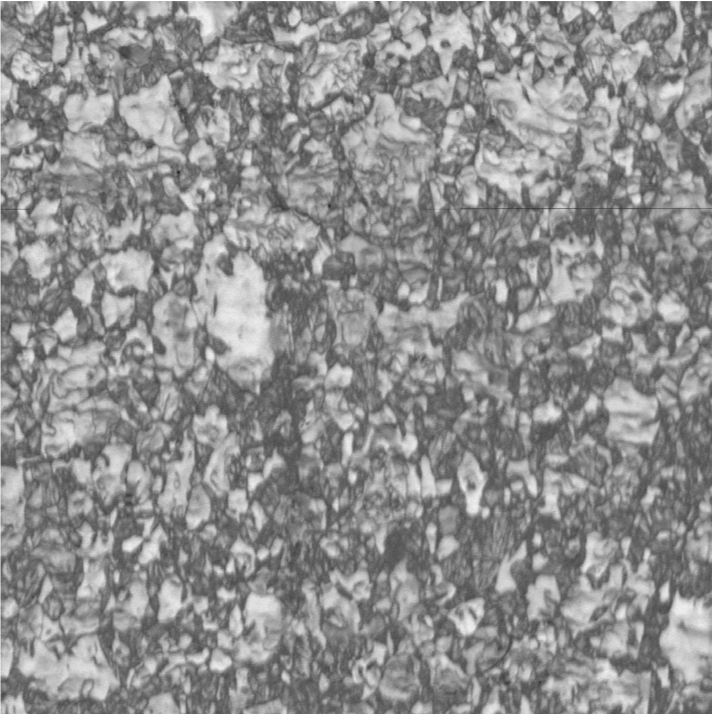
\includegraphics[width=\textwidth]{Micro1_980.png}
         \caption{}
         \label{fig:Micro1_980}
     \end{subfigure}
     \hfill
     \begin{subfigure}[b]{0.3\textwidth}
         \centering
         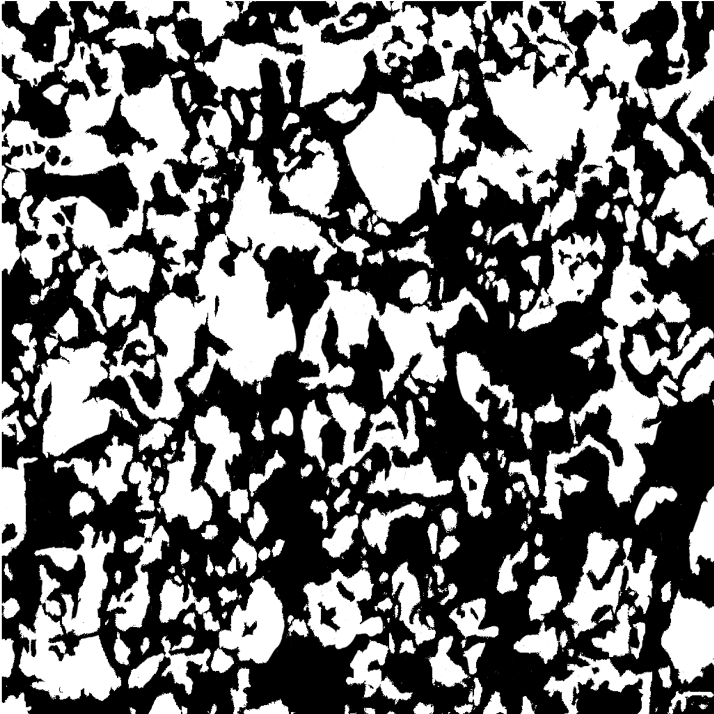
\includegraphics[width=\textwidth]{Micro2_980.png}
         \caption{}
         \label{fig:Micro2_980}
     \end{subfigure}
          \hfill
     \begin{subfigure}[b]{0.3\textwidth}
         \centering
         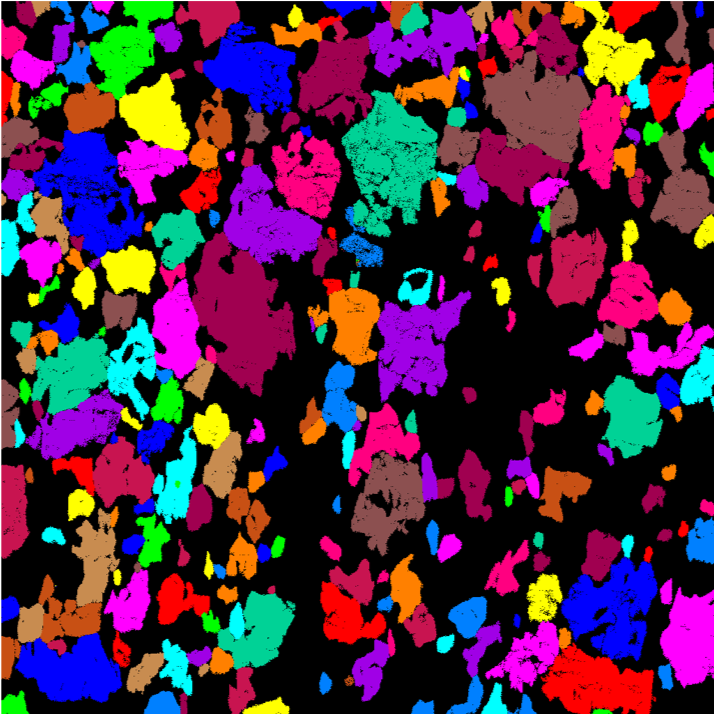
\includegraphics[width=\textwidth]{Micro3_980.png}
         \caption{}
         \label{fig:Micro3_980}
     \end{subfigure}
     \caption{Microstructure of DP980}
     \label{fig:Micro_980}
\end{figure}

As can be seen both from fig. \ref{fig:Micro_500}-\ref{fig:Micro_980} and table \ref{tab:MicrostructurePara} the ferritic grain sizes are decreasing with increasing volume fraction of martensite. The martensite grain sizes are decreasing from DP500 to DP800, but with DP980 comes an increase. DP980 also has an much larger martensite volume fraction compared to the other three steel grades. 

\begin{center}
\begin{table}[h!]
    \centering

    \begin{tabular}{c|cccccc}
    \hline
         & $d_m [\mu m]$ & $d_f [\mu m]$ & $L_m [\mu m]$ & $L_f [\mu m]$& $V_m [\%]$& $V_f [\%]$ \\ [0.5ex]
         \hline
         \rowcolor{Gray}
         DP500 & $3.41 \pm 2.74$ & $8.4 \pm 6.4$ & $2.5 \pm 0.4$& $15.8 \pm 2.4$ & $14 \pm 0.3$ & $86 \pm 0.3$ \\
         
         DP600 &$2.27 \pm 1.26$ & $3.5 \pm 2.4$ & $1.5 \pm 0.1$& $6.9 \pm 0.5 $& $18 \pm 2.2$ & $82 \pm 2.2 $\\
         \rowcolor{Gray}
         DP800 &$1.94 \pm 2.15$& $3.3 \pm 2 $&$1.5 \pm 0.2 $& $3.9 \pm 0.5$ & $28 \pm 3.2$ &$72 \pm 3.2$ \\
         
         DP980 &$2.47 \pm 8.45 $& $2.7 \pm 2.1 $&$7.8 \pm 0.7 $& $ 6.8 \pm 1$ &$54 \pm 1.3$ & $46\pm 1.3 $\\
         \hline
    \end{tabular}
    \caption{Microstructure parameters}
    \label{tab:MicrostructurePara}
\end{table}
\end{center}



The chemical composition was given by the steel producer, SSAB, and is given in table \ref{tab:ChemicalComp}.

Ferrite has a considerable lower carbon saturation point compared to martensite. It is therefore commonly assumed that the ferrite in DP-steels is supersaturated, \cite{Calcagnotto2},\cite{Granbom}. At room temperature the ferritic carbon content is then, according to [4-5] $C_f=0.008$. It is then further assumed that the rule of mixture is applicable:

\begin{equation}
\label{Eq:RuleofMix}
  C_{tot} = C_f*V_f + C_m*V_m  
\end{equation}

Such that the carbon content in the martensite may be computed as:

\begin{equation}
\label{Eq:CalcFracMart}
  C_{m} = \frac{C_{tot}-C_f*V_f }{V_m}
\end{equation}


\begin{center}
\begin{table}[]
    \centering
    \begin{tabular}{c|cccc}
    \hline
         & C & Nb & Mn & Si  \\ [0.5ex]
         \hline
         \rowcolor{Gray}
         DP500 & 0.079 & 0 & 0.7& 0.3 \\
         
         DP600 &0.094 & 0.015 & 0.9& 0.2 \\
         \rowcolor{Gray}
         DP800 &0.136 &0.016 & 1.6&0.2 \\
         
         DP980 &0.144 &0.015 &1.5 &0.19 \\
         \hline
    \end{tabular}
    \caption{Chemical composition}
    \label{tab:ChemicalComp}
\end{table}
\end{center}



\subsection{Mechanical properties}
\subsubsection{Tensile test}
Standard tensile tests were performed according to the procedure described in section \ref{Section:Tensiletest} for all of the four DP-steels. Four tests where performed for each steel. The geometry of the specimens are given in fig. \ref{fig:SpecimenDim}. The thickness was 2 mm for all of the steels except for DP500 which was only 1 mm. To obtain stress-strain curves from the test, DIC (Digital Image Correlation) was used. The specimens were painted in a black and white speckle pattern prior to the tests. A high frequency camera is used during the tests, taking about ??? frames per second. These images are then analysed in the software eCorr. Some characteristic points in the speckle pattern are identified and then traced during the deformation through the series of frames. From the obtained force-displacment curve, engineering stress-strain and then true stress and strain curve can be calculated from equation \ref{Eq:EngStressStrain} and \ref{Eq:TrueStressStrain}. 
\begin{figure}[h!]
\centering
    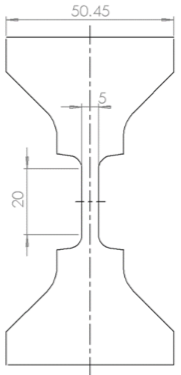
\includegraphics[width=0.3\linewidth]{SpecimenDim.png}
    \caption{Dimensions of specimen used in tensile test}
    \label{fig:SpecimenDim}
\end{figure}

Tensile tests according to 
\begin{figure}[h!]
\centering
    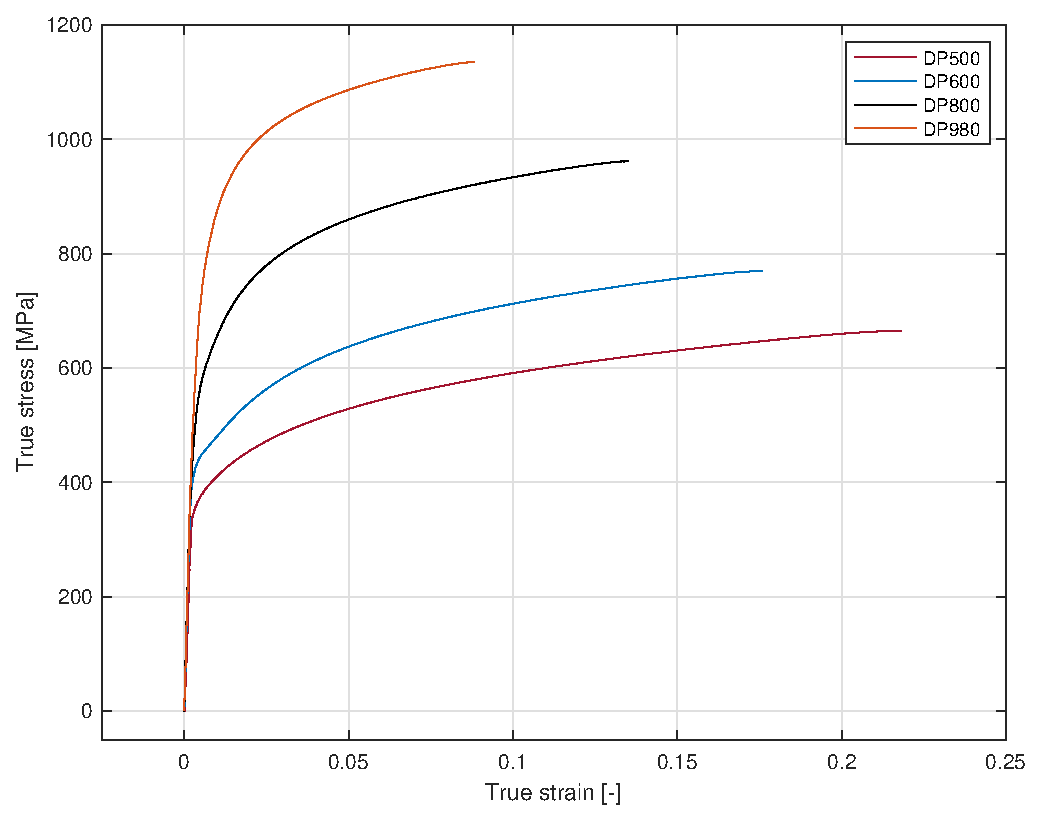
\includegraphics[width=0.8\linewidth]{Experimental.eps}
    \caption{Results from tensile tests}
    \label{fig:TensiletestResult}
\end{figure}

\subsubsection{Hardness}


\section{Numerical model - Results and Validation}
\subsection{Plastic deformation}
\label{Section:PlasticDeform}
Micromechanical simulations were performed with the RVE presented in section \ref{Section:Axisym}, simplified to an axisymetric model when implemented in ABAQUS. Respective single phase material model described in section \ref{Micromodel} was applied to each phase in the model. Without any fitting of parameters to the experimental results, but only with the use of the values used by \cite{Ramazani} and by not including the Hall-Petch strengthening for the martensite (since it is uncertain what should be taken as "grain size"), the following results were obtained:

\begin{figure}[h!]
     \centering
     \begin{subfigure}[b]{0.45\textwidth}
         \centering
         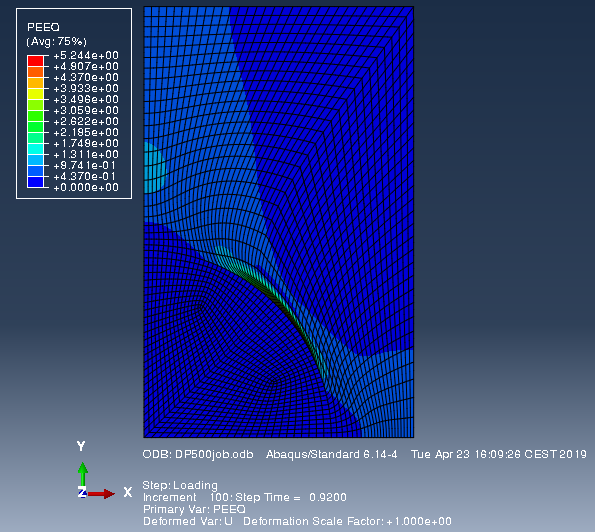
\includegraphics[width=\textwidth]{PlastStrain500.png}
         \caption{}
         \label{fig:PlastStrain500}
     \end{subfigure}
     \begin{subfigure}[b]{0.45\textwidth}
         \centering
         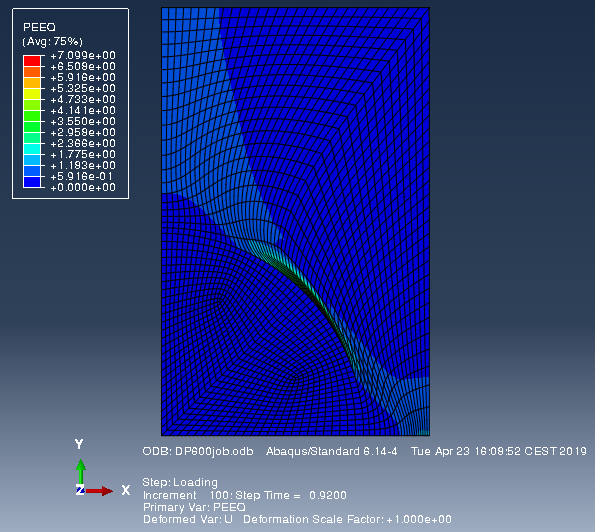
\includegraphics[width=\textwidth]{PlastStrain600.png}
         \caption{}
         \label{fig:PlastStrain600}
     \end{subfigure}
          \hfill\\
     \begin{subfigure}[b]{0.45\textwidth}
         \centering
         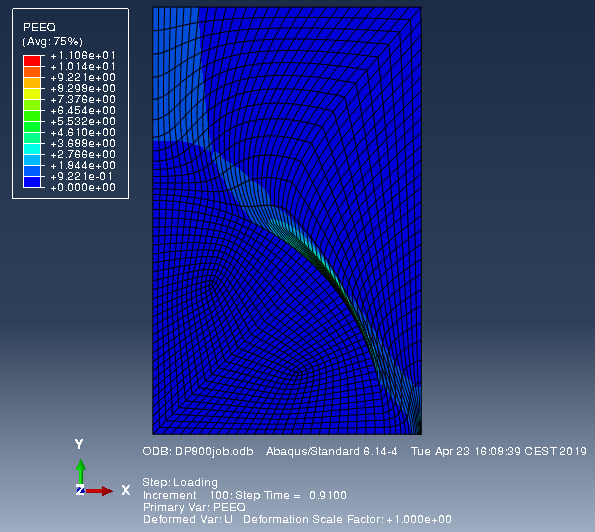
\includegraphics[width=\textwidth]{PlastStrain800.png}
         \caption{}
         \label{fig:PlastStrain800}
     \end{subfigure}
     \begin{subfigure}[b]{0.45\textwidth}
         \centering
         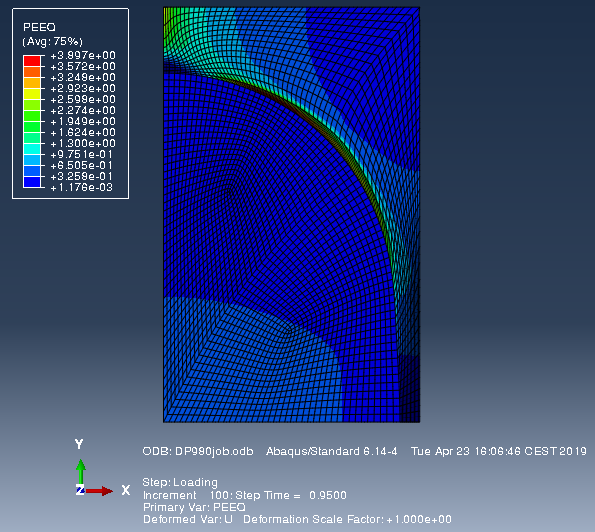
\includegraphics[width=\textwidth]{PlastStrain980.png}
         \caption{}
         \label{fig:PlastStrain980}
     \end{subfigure}
     \caption{}
     \label{fig:PlasticStrain}
\end{figure}

The response is similar for all four steels. Equivalent plastic strain initiate at the grain boundary between martensite and ferrite. This is also where the highest values of the plastic strain is obtained, which is shown in fig. \ref{fig:PlastStrain500}- \ref{fig:PlastStrain980} and also fig. \ref{fig:PEEQvsDist} where the equivalent plastic strain in the elements along the diagonal in the model is plotted against the distance from origo along the r-axis, for DP500. As can be seen the high strain is very local, only about 3 \% of the total length of the model experiences the high strains.



\begin{figure}[!h]
  \centering
  \begin{minipage}[b]{0.4\textwidth}
    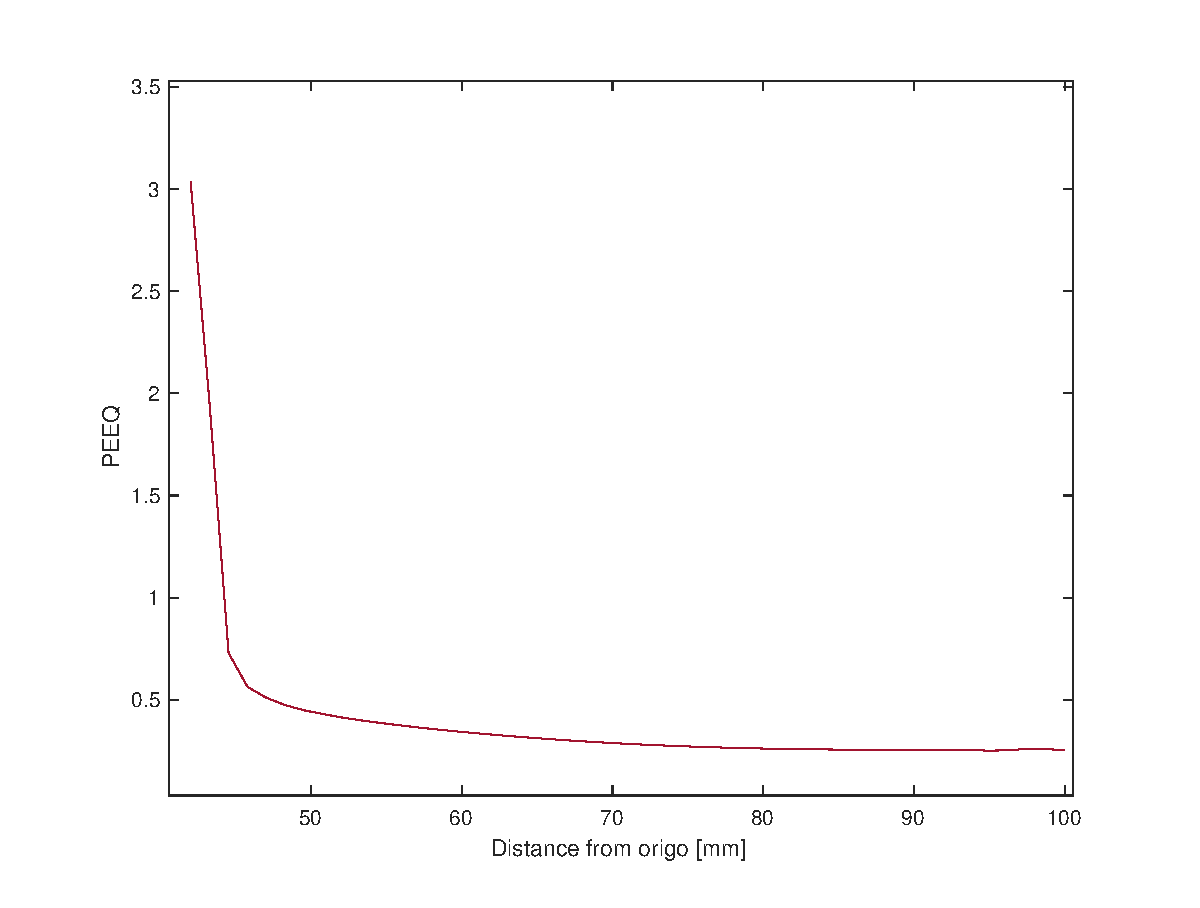
\includegraphics[width=\textwidth]{PEEQvsDist.eps}
    \caption{Equivalent plastic strain along diagonal in the ferrite. }
    \label{fig:PEEQvsDist}
  \end{minipage}
  \hfill
  \begin{minipage}[b]{0.4\textwidth}
    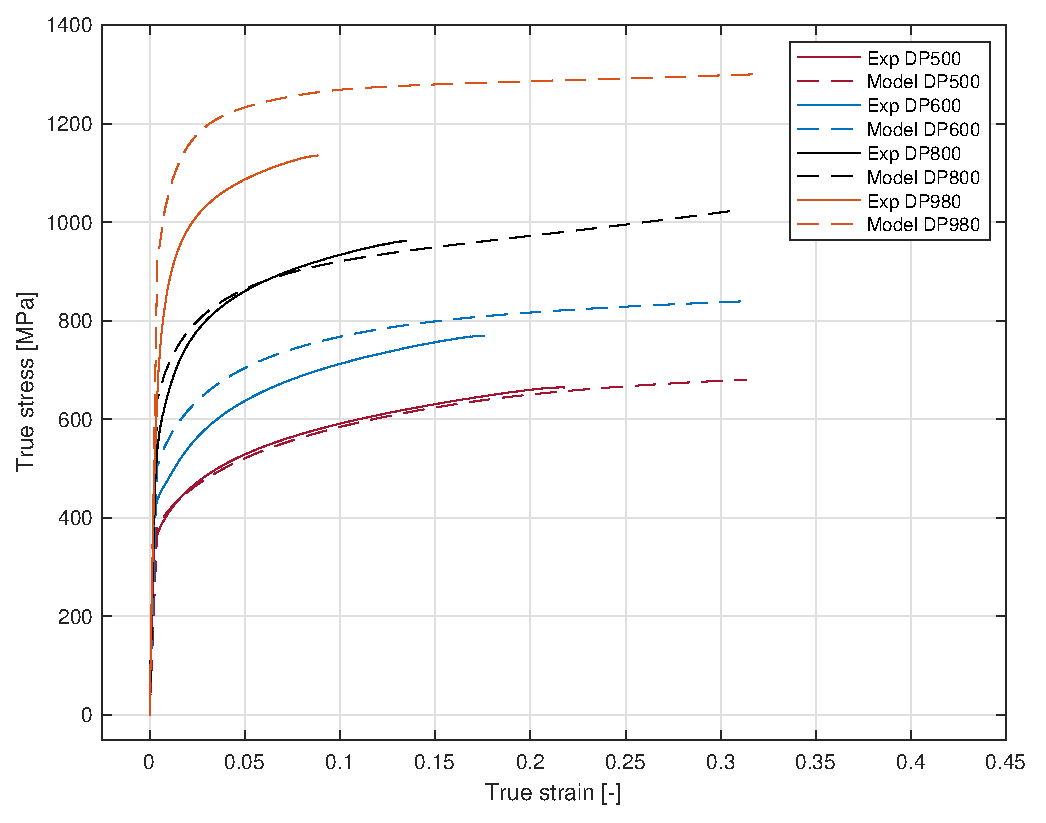
\includegraphics[width=\textwidth]{MeanMean.eps}
    \caption{Experimental results vs. Numerical results}
  \end{minipage}
\end{figure}

Only DP980 experience plastic strain in the martensite. This is visualised as the lighter blue field in the lower left corner in \ref{fig:PlastStrain980}. That only the steel with a high volume fraction of martensite do deform plastically is a result in accordance with the outcome of the research made by \cite{Al-Abbasi2003}. They used the same axisymmetrical model as in this work, and studied the difference in the radius of the martensitic sphere. 

When comparing to experimental results in the stress strain curves in fig. \ref{fig:} an overall precise fit is obtained for DP500, DP600 and DP800. DP980 though, show too high values of stress in the numerical result. 

The model can be improved and further calibration and fitting of parameters is needed. A sensitivity study is performed to see how sensitive the model is to changes in different input parameters. Variations in carbon content, grain size and mesh will be studied. 
 

\subsection{Sensitivity study - Carbon content}
\label{SensStudyCarbon}

To see how and to which magnitude the carbon content affects the material behaviour the point of supersaturation in the ferrite is changed with +/- 0.002 wt\%. The total carbon content will be kept constant.  

\begin{figure}[h!]
     \centering
     \begin{subfigure}[b]{0.3\textwidth}
         \centering
         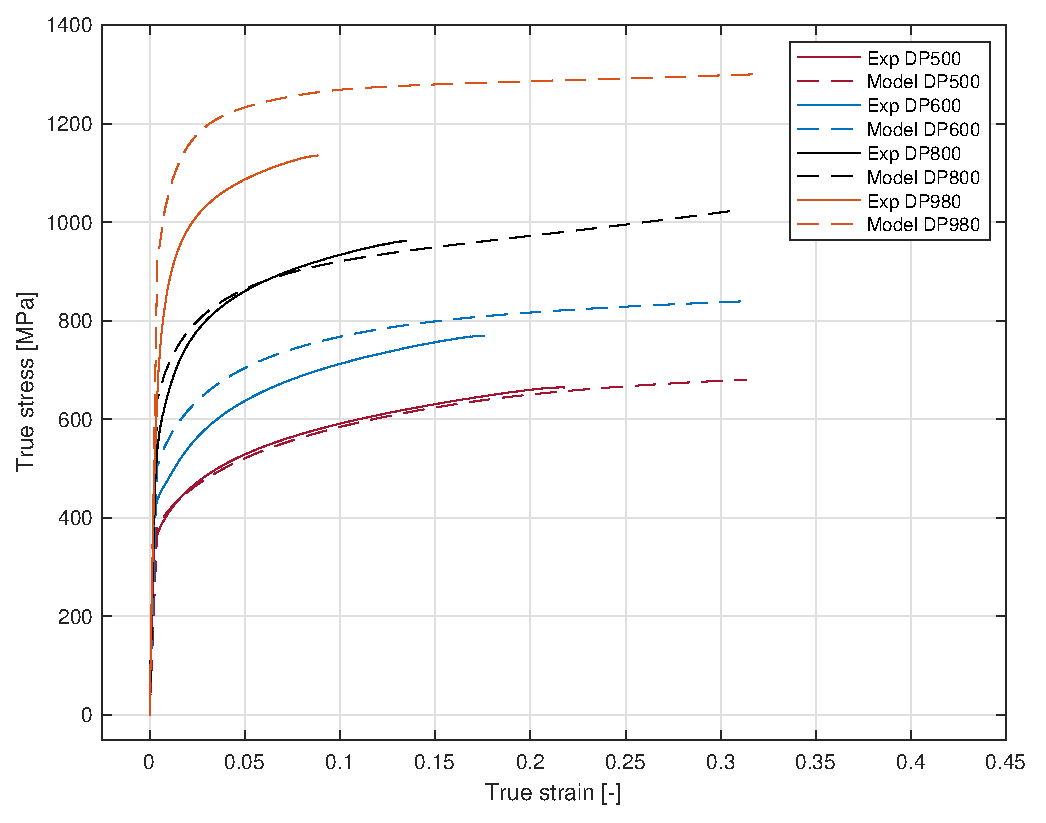
\includegraphics[width=\textwidth]{MeanMean.eps}
         \caption{Mean value $C_f$=0.008}
         \label{fig:CarbonMean}
     \end{subfigure}
     \hfill
     \begin{subfigure}[b]{0.3\textwidth}
         \centering
         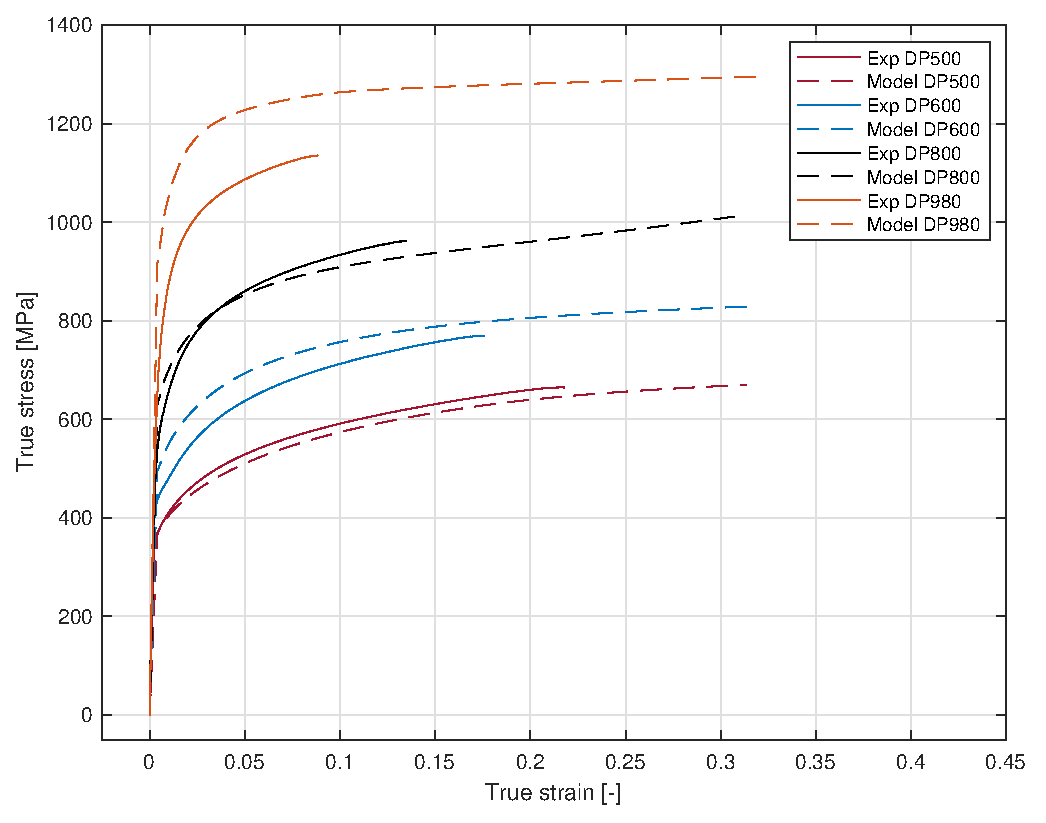
\includegraphics[width=\textwidth]{CarbonMin.eps}
         \caption{Min value $C_f$=0.006}
         \label{fig:CarbonMin}
     \end{subfigure}
          \hfill
     \begin{subfigure}[b]{0.3\textwidth}
         \centering
         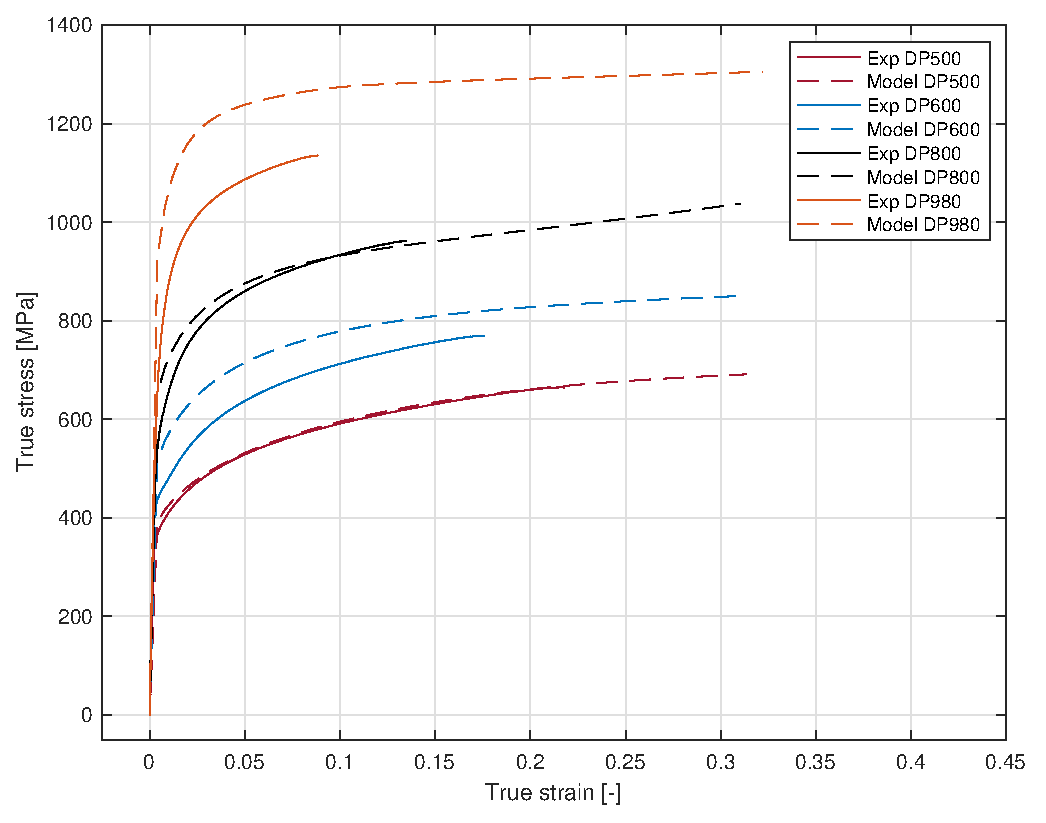
\includegraphics[width=\textwidth]{CarbonMax.eps}
         \caption{Max value $C_f$=0.01}
         \label{fig:CarbonMax}
     \end{subfigure}
     \caption{Sensitivity study of carbon content}
     \label{fig:CarbonContent}
\end{figure}

As can be seen in fig.\ref{fig:CarbonContent} the variation in carbon content only has small effect on the mechanical behaviour of all the four steel grades. The total carbon content was, as described, kept constant and only $C_f$ varied, which according to equation \ref{Eq:RuleofMix} lead to variations in $C_m$ as well. But these changes will only be reflected in DP980 since no yielding of martensite occurs in DP500-DP800. 
Further studies of the relationship between carbon and the strengthening of martensite can be found in section \ref{MartensiteCarbon} where the constants in equation \ref{solidsolM}


\subsubsection{Sensitivity study - Grain size}
\label{SensStudyGrain}
The sensitivity study of the grain size is done by using the extreme values in the reported range of grain sizes. Since only DP980 exhibit plastic flow, only the ferritic grain size will be varied. 

\begin{figure}[h!]
     \centering
     \begin{subfigure}[b]{0.3\textwidth}
         \centering
         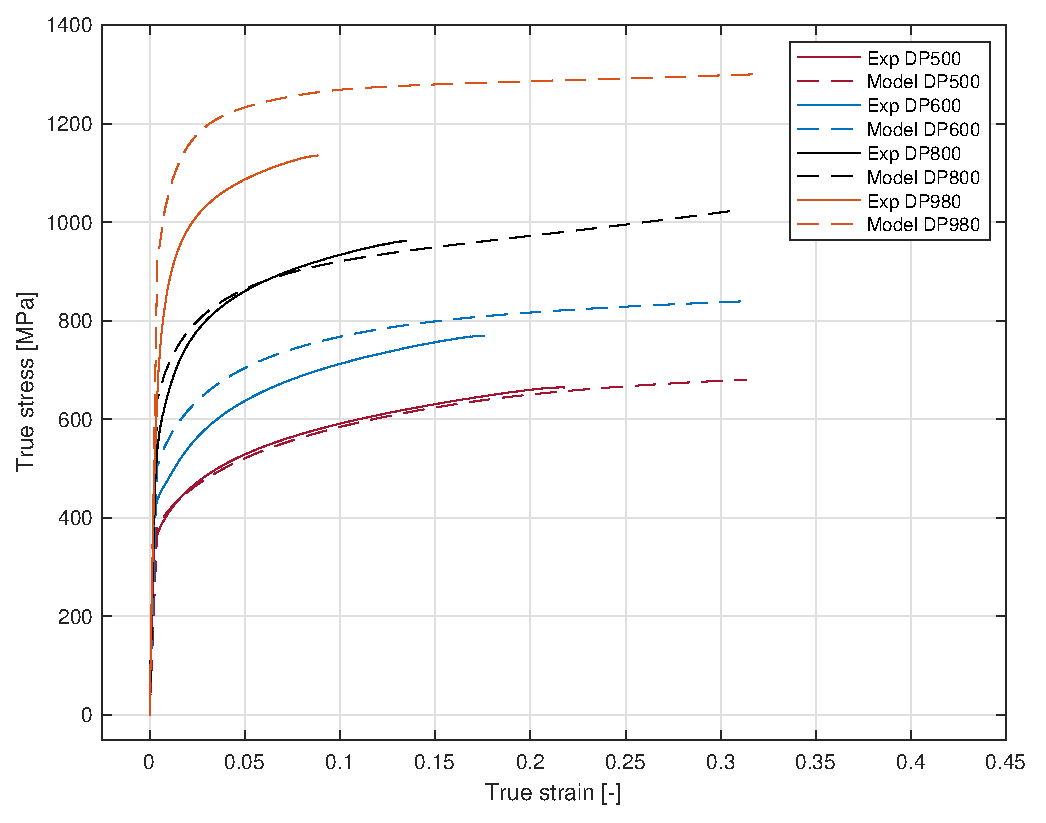
\includegraphics[width=\textwidth]{MeanMean.eps}
         \caption{Mean value $d_f$}
         \label{fig:Mean}
     \end{subfigure}
     \hfill
     \begin{subfigure}[b]{0.3\textwidth}
         \centering
         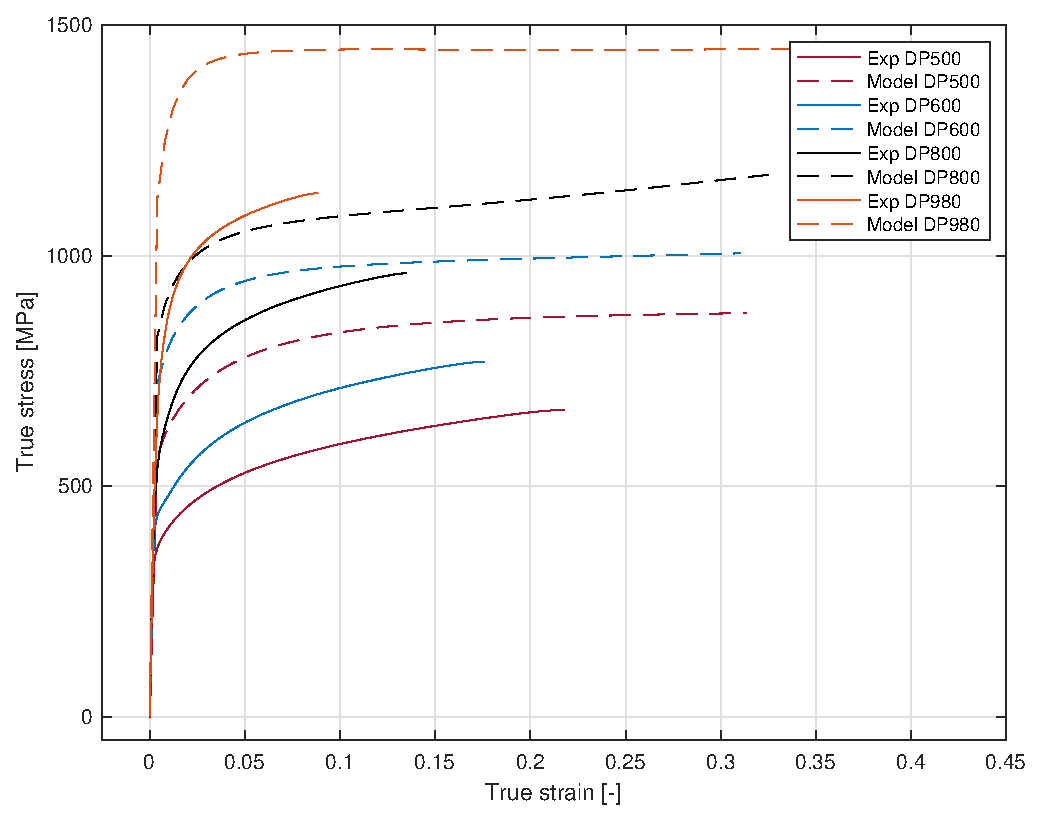
\includegraphics[width=\textwidth]{GrainMin.eps}
         \caption{Min value $d_f$}
         \label{fig:GrainMin}
     \end{subfigure}
          \hfill
     \begin{subfigure}[b]{0.3\textwidth}
         \centering
         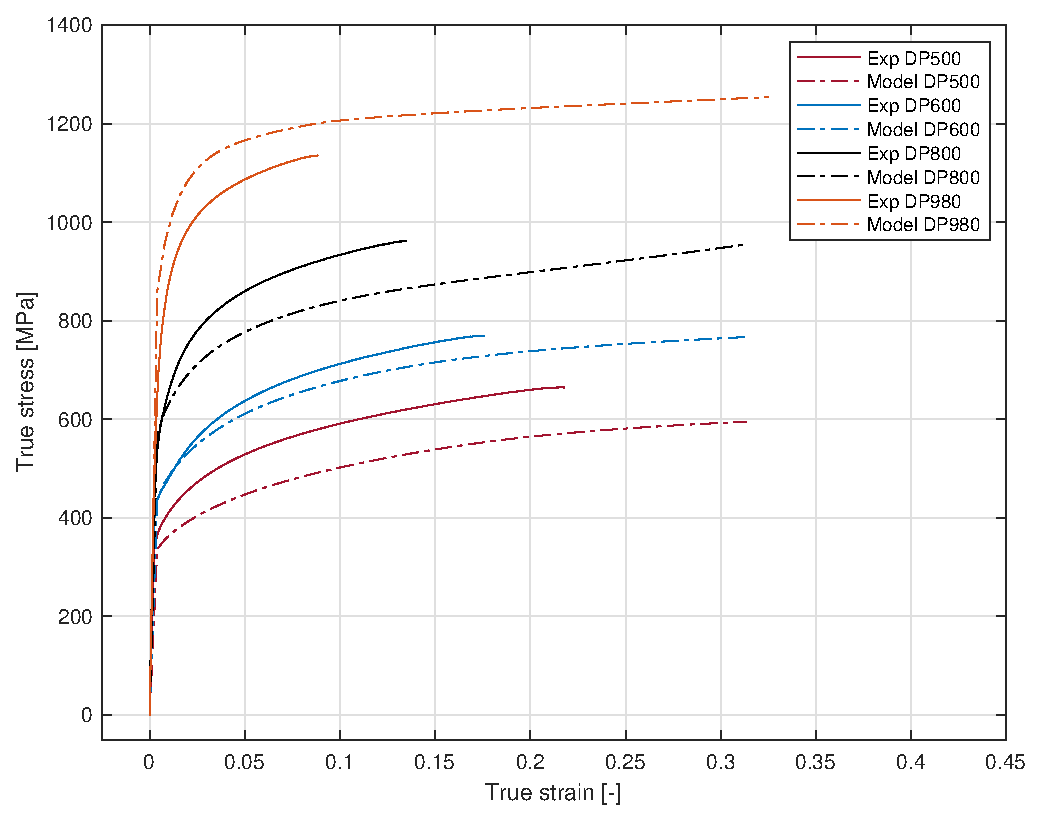
\includegraphics[width=\textwidth]{GrainMax2.eps}
         \caption{Max value $d_f$}
         \label{fig:GrainMax}
     \end{subfigure}
     \caption{Sensitivity study of grain size}
     \label{fig:GrainSize}
\end{figure}

It is evident that the ferritic grain size do affect the response, in comparison to the carbon content and mesh size, to a great extent. This is also reported frequently in the litterature, e.g. by \cite{Mazaheri} and ????. For ferrite, the grain size is a factor affecting both the Hall-Petch strenghtening and the strain hardening since the free path $L_f$ is taken equal as the grain size $d_f$. Smaller grain size lead to an overestimation of the plastic flow, while larger grains give an underestimation. This is explained by the grain boundary strengthening where smaller grains increase the total length of grain boundaries and also an increase of dislocations that origin from the volume expansion during the transformation from austenite to martensite. 

\begin{figure}[h!]
     \centering
     \begin{subfigure}[b]{0.45\textwidth}
         \centering
         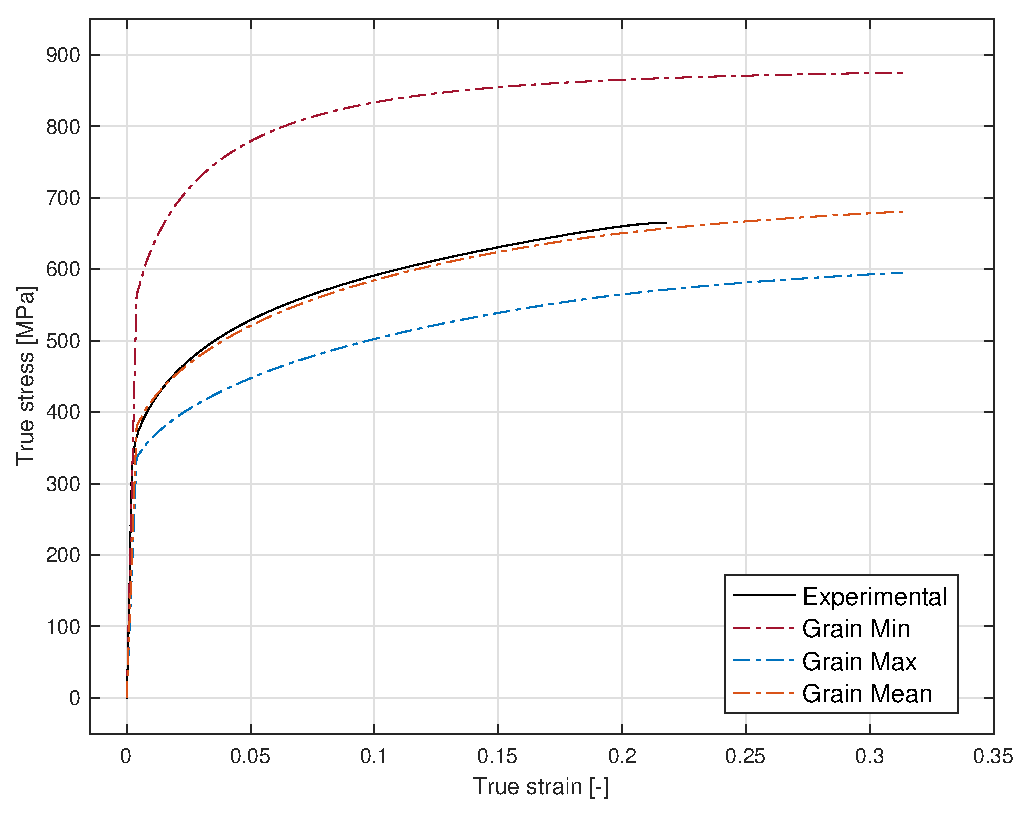
\includegraphics[width=\textwidth]{Grain500.eps}
         \caption{DP500}
         \label{fig:Grain500}
     \end{subfigure}
     \begin{subfigure}[b]{0.45\textwidth}
         \centering
         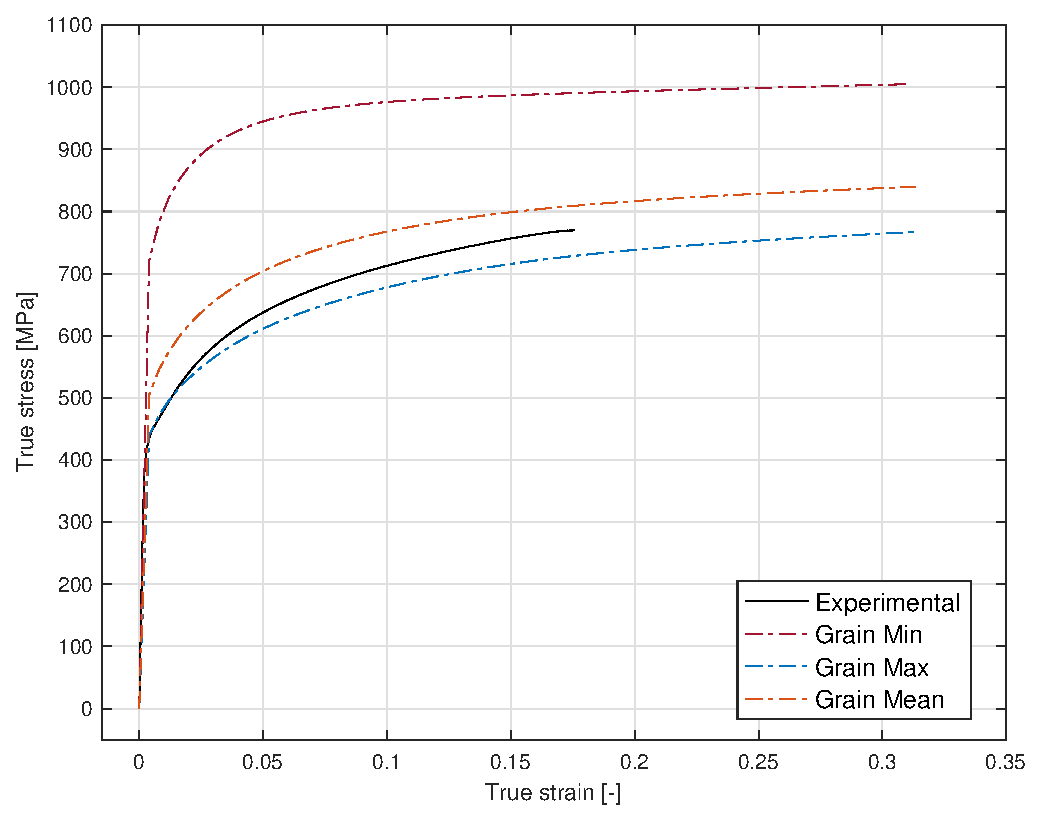
\includegraphics[width=\textwidth]{Grain600.eps}
         \caption{DP600}
         \label{fig:Grain600}
     \end{subfigure}
          \hfill\\
     \begin{subfigure}[b]{0.45\textwidth}
         \centering
         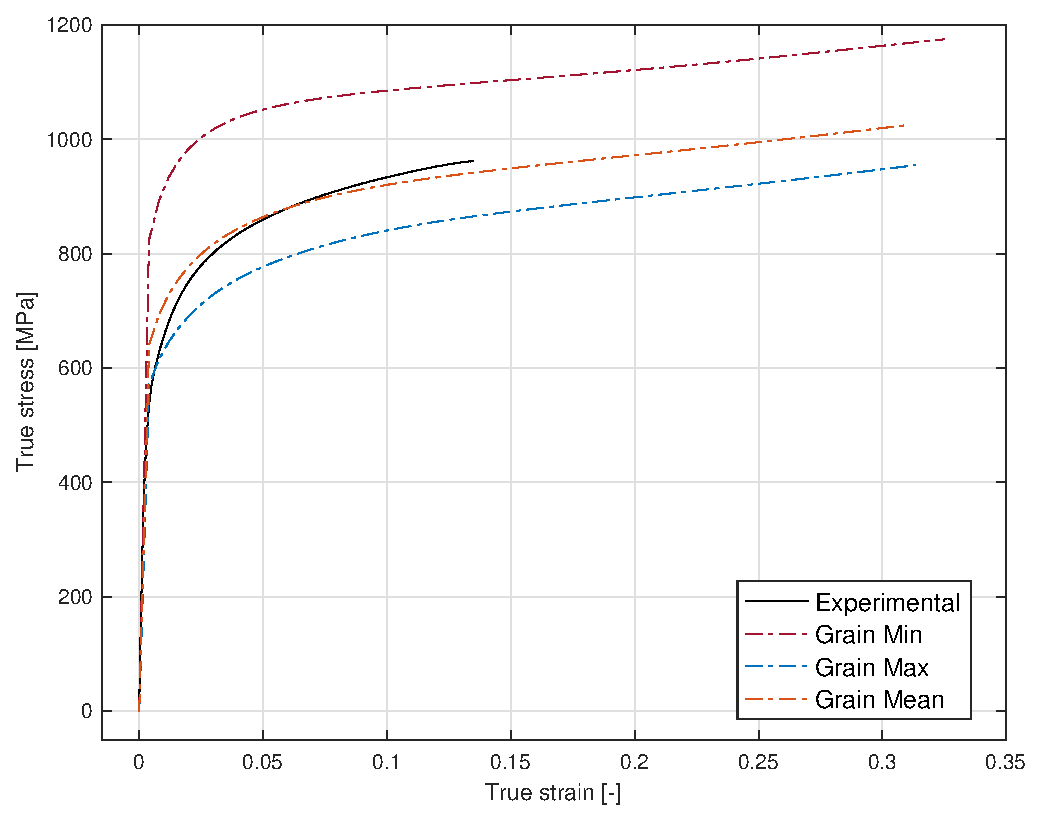
\includegraphics[width=\textwidth]{Grain800.eps}
         \caption{DP800}
         \label{fig:Grain800}
     \end{subfigure}
     \begin{subfigure}[b]{0.45\textwidth}
         \centering
         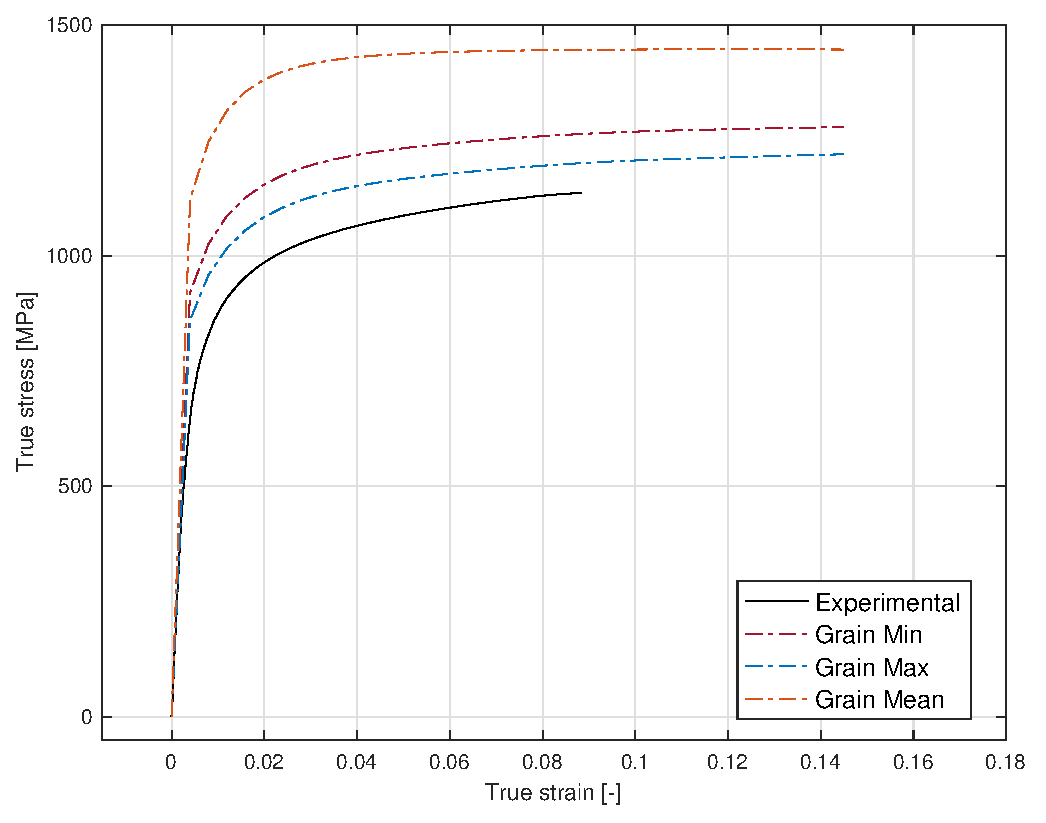
\includegraphics[width=\textwidth]{Grain980.eps}
         \caption{DP980}
         \label{fig:Grain980}
     \end{subfigure}
     \caption{Grain size variation}
     \label{fig:GrainVariation}
\end{figure}
For the validation of the numerical model, it can be seen from fig. \ref{fig:GrainVariation} that the experimental result is within the spread of ferritic grain sizes, for all of the steels except DP980. All the numerical results for DP980 are over-estimations. This implies that with the exact true value of the ferritic grain size the model could possibly represent the true flow curve for ferrite, while yet another indication on that the martensite is not properly represented is obtained, since non of the values within the standard deviation of ferritic grain size will give the correct response. 

\subsubsection{Sensitivity study - Mesh}
\label{SensStudyMesh}
To investigate if the mesh size has an effect on the result, the mesh size was both increased and decreased. The number of elements in each case can be seen in table \ref{tab:NumberElem} and the response from the study in fig. \ref{fig:Mesh}.



\begin{center}
\begin{table}[h!]
    \centering
    \begin{tabular}{c|ccc}

        \hline
         & Mean & Min & Max  \\ [0.5ex]
         \hline
         \rowcolor{Gray}
         DP500 & 2526 & 672 & 5616 \\
         
         DP600 &2218 & 4840 & 562 \\
         \rowcolor{Gray}
         DP800 &1729 & 3760 &434  \\
       
         DP980 &3455 &4194 &691 \\
         \hline

    \end{tabular}
    \caption{Number of elements in mesh}
    \label{tab:NumberElem}
\end{table}
\end{center}

\begin{figure}[h!]
     \centering
     \begin{subfigure}[b]{0.3\textwidth}
         \centering
         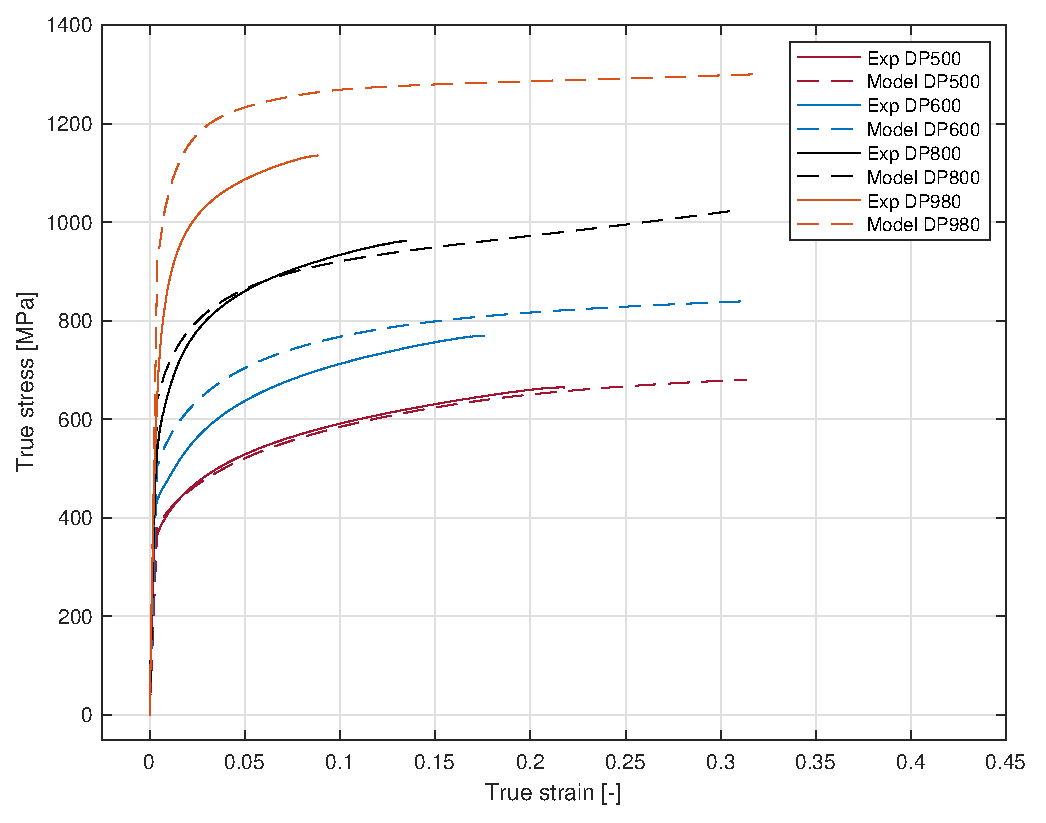
\includegraphics[width=\textwidth]{MeanMean.eps}
         \caption{Mean value number of elements}
         \label{fig:MeshMean}
     \end{subfigure}
     \hfill
     \begin{subfigure}[b]{0.3\textwidth}
         \centering
         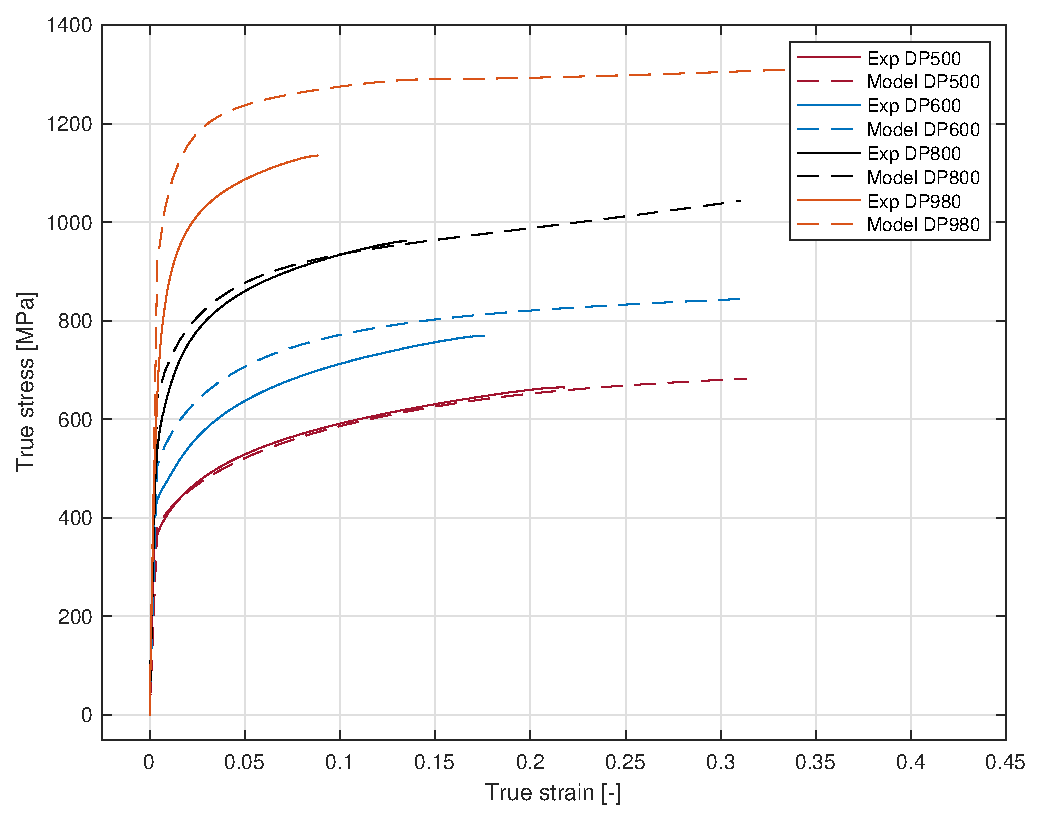
\includegraphics[width=\textwidth]{MeshMin.eps}
         \caption{Min value number of elements}
         \label{fig:MeshMin}
     \end{subfigure}
          \hfill
     \begin{subfigure}[b]{0.3\textwidth}
         \centering
         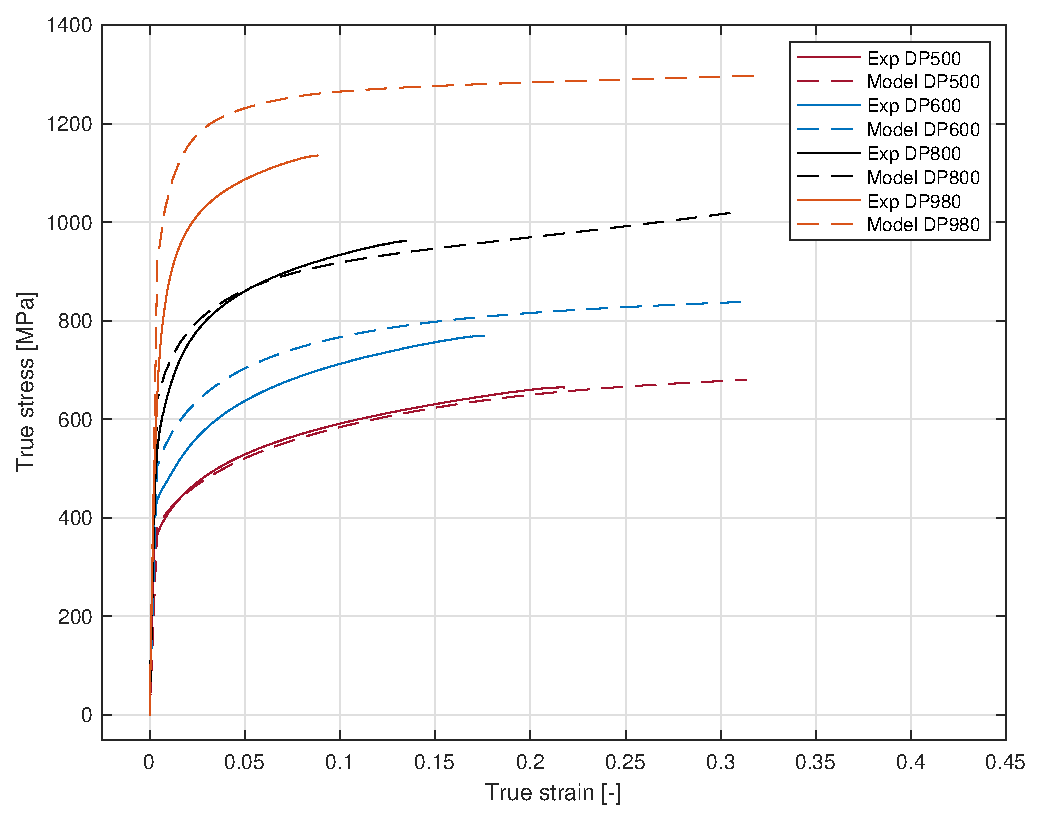
\includegraphics[width=\textwidth]{MeshMax.eps}
         \caption{Max value number of elements}
         \label{fig:MeshMax}
     \end{subfigure}
     \caption{Sensitivity study of mesh size}
     \label{fig:Mesh}
\end{figure}

The number of elements has a minor effect on the result. Therefore the larger element sizes could be used to decrease the computational cost without any loss in quality. However, since the model already is computational effective with sufficiently short running time (about 30 s) the mean number of elements will be used further. 

\subsubsection{Discussion}
The numerical results for the three lower steel grades give a good fit to the experimental data and in addition have in common that the martensite do not plastically deform in the simulations. The DP980 however, show a large deviation in the numerical result from the experimental and in addition the martensite starts to yield in the simulations. This implies that the model is able to represent the ferritic phase precisely, while the martensitic model need further studies and modifications. 

From the three sensitivity studies and fig. \ref{fig:CarbonContent} and \ref{fig:Mesh}, it is clear that variations in carbon content and the number of elements in the mesh has minor effect on the result. This in contrast to the effect of changes in the ferrite grain size. 

Calibration of the martensitic phase is needed and from the sensitivity study it is evident that studies on the grain size and the Hall-Petch strengthening should be prioritized. 

Even thought the sensitivity study of carbon did not show any large effect on the plastic flow, it is not excluded that the equation describing the solid solution strengthening from carbon (eq. \ref{solidsolM}) might need to be improved and that that change will have a larger effect on the flow curve.  

\subsubsection{Calibration of Martensite}
\label{MartensiteCarbon}
Apart from the four DP-steels, three pure martensitic steels, 1200M, 1400M and 1700M, have been tested, both in hardness and tensile tests. The results from these tests have been used to study the martensite as a single phase, as it is difficult to separate the ferrite and the martensite and the interaction between the two phases in the results from the DP-steels.

The result from the hardness tests on the martensitic steel has been plotted against the carbon content in the same steels. A close to linear relationship between the two parameters was found. From a linear fitting of this relation, the carbon content in the martensite in DP980 was used to approximate the hardness of the martensite in DP980. This hardness value of 586 HV was then used in the plot of hardness versus yield stress in the martensitic steels, to find the yield stress of martensite in DP980. The resulting value was 1234 MPa. The process is illustrated in fig. \ref{fig:ValidationMart}. Since it is not possible to separate the martensitic yield stress in the experimental results of DP980, this value can not be used to validate the relationship between the martensite in the martensitic steel and the DP steel. What can be compared though is the yield stress of martensite in the DP steel according to the numerical model. 
\begin{figure}[h!]
    \centering
    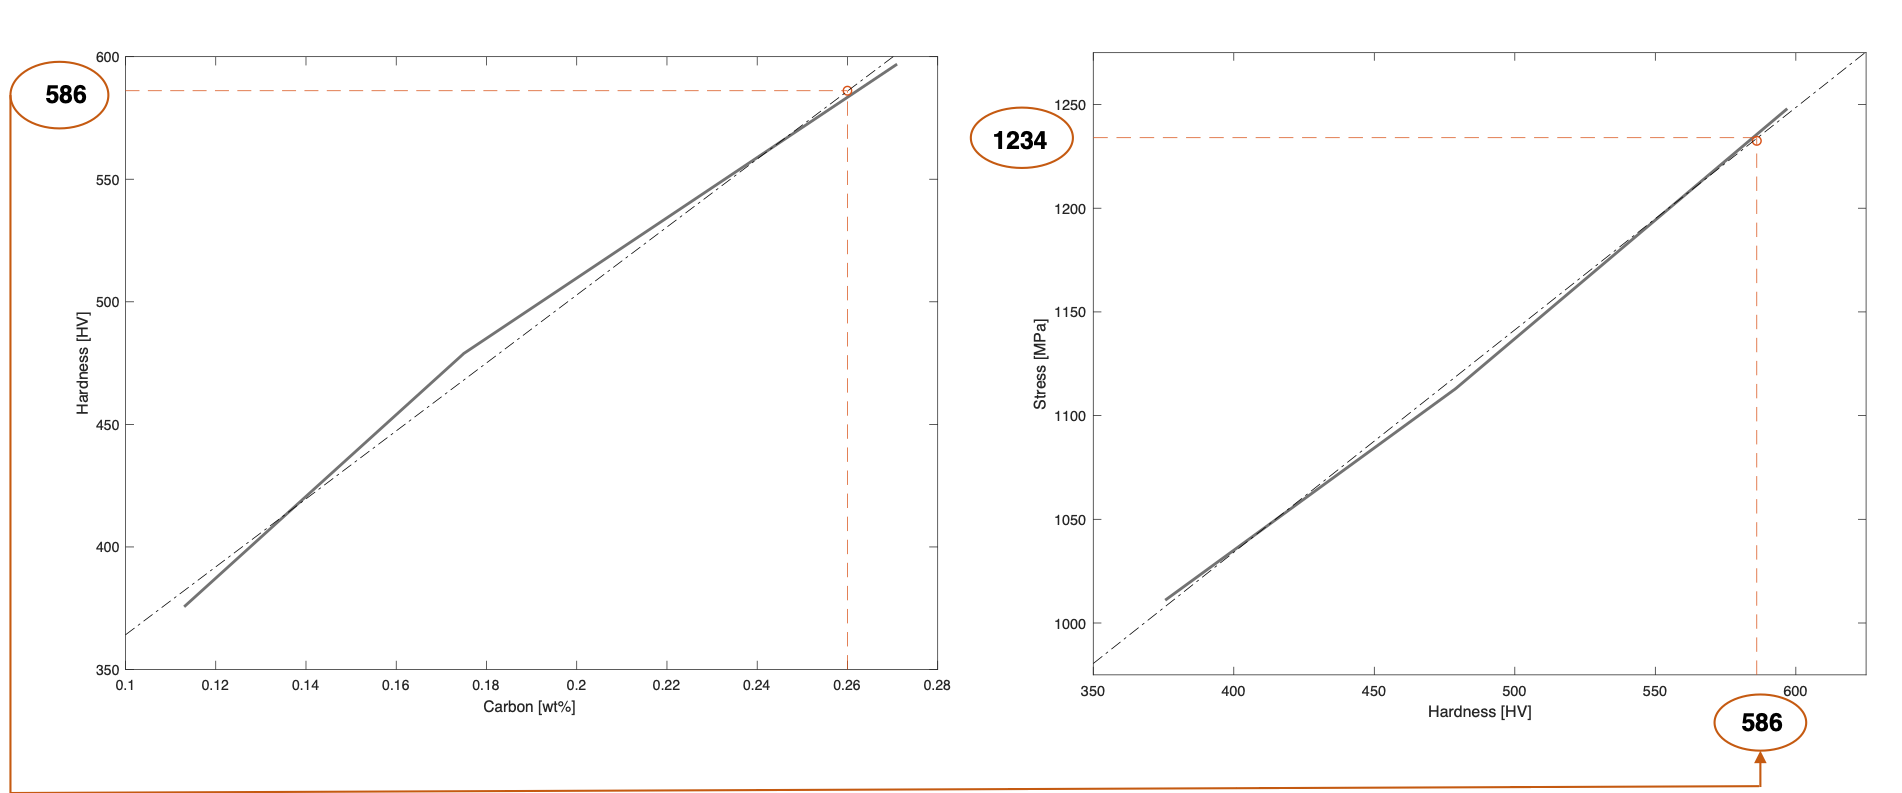
\includegraphics[width=\linewidth]{ValidationMart.png}
    \caption{Yield stress of martensite in DP-steel according to relationships based on martensitic steels}
    \label{fig:ValidationMart}
\end{figure}

The calculated plastic flow according to equation \ref{Eq:Flowstress} for each phase and for all DP-steel grades is shown in fig. 

\begin{figure}[h!]
    \centering
    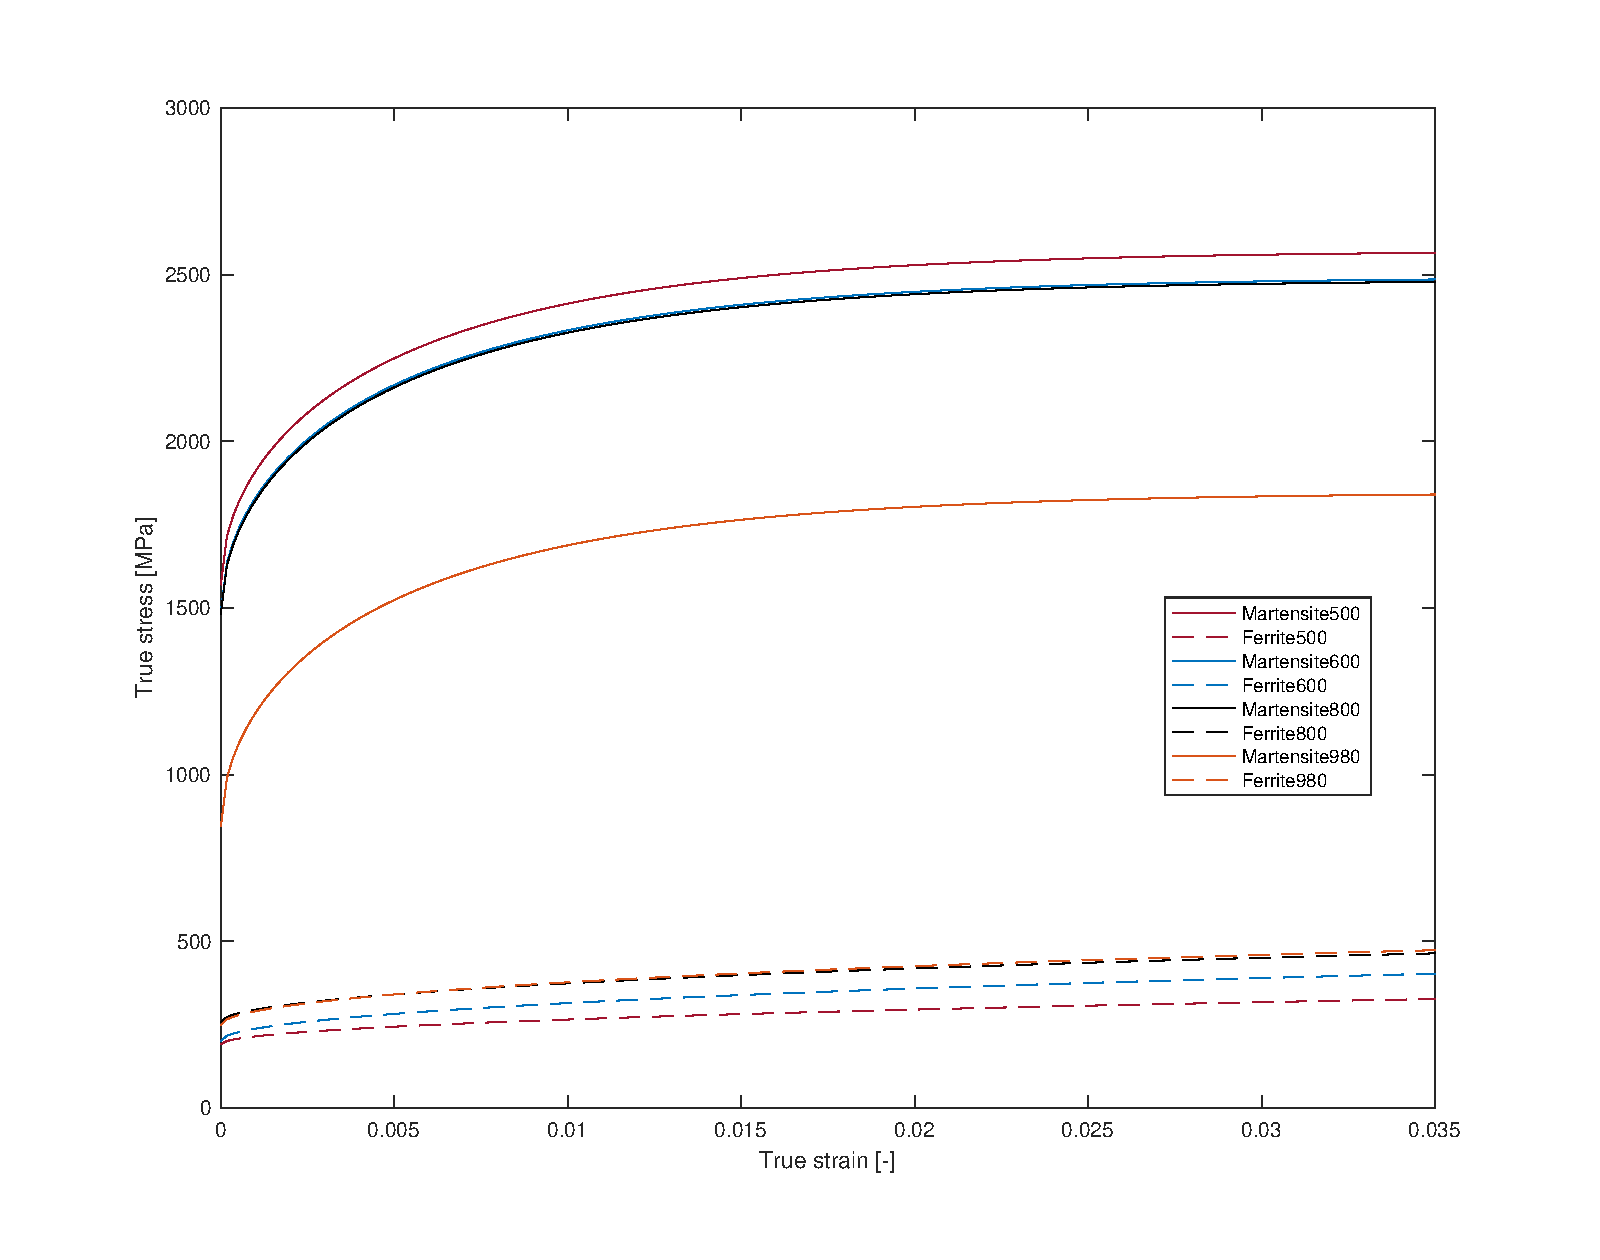
\includegraphics[width=\linewidth]{PhaseYield.eps}
    \caption{Plastic flow curve for single phases.}
    \label{fig:PhaseYield}
\end{figure}

Interesting is that the plastic flow of the martensitic phase for DP980 is considerably lower than for the three lower steel grades. The ferritic phases are more homogenized for all of the steels and the ranking in strength corresponds well with the ranking in total strength of the materials. The reason why the DP980 even though the relative low strength of the martensite, in the total response is the strongest steel, is due to the volume fraction of martensite. If the stress components are multiplied with respective volume fraction of each phase in order to get the relative contribution from each phase to the total response, the result given in fig. \ref{fig:PhaseYieldFrac} is obtained. Now the ranking of strength in martensite correspond to the overall strength of the steels.

\begin{figure}[h!]
    \centering
    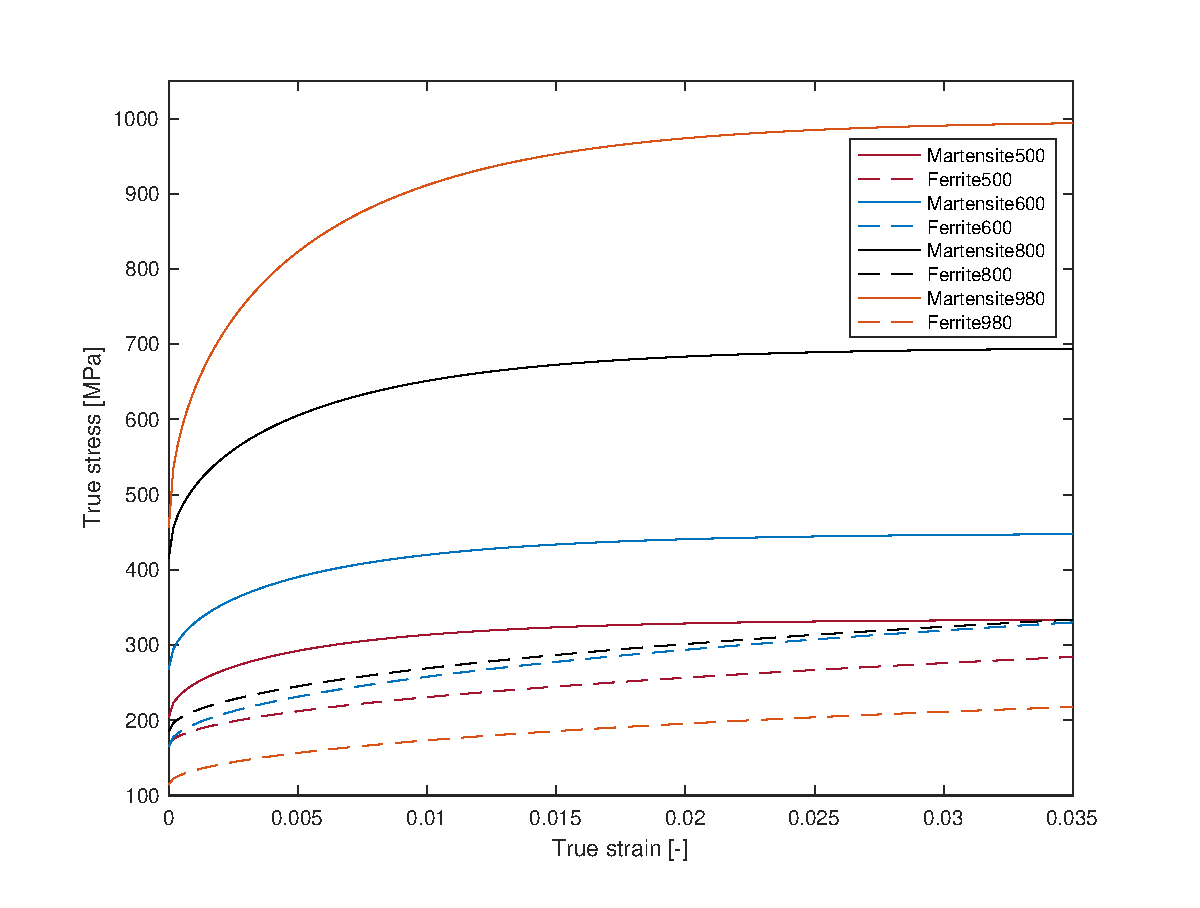
\includegraphics[width=\linewidth]{PhaseYieldFrac.eps}
    \caption{Plastic flow curve for single phases when multiplied with respective volume fraction of phase.}
    \label{fig:PhaseYieldFrac}
\end{figure}




\subsection{Ductile fracture}
Due to the ductile behavior of the ferrite the most likely fracture mechanism is assumed to be ductile fracture as a consequence of nucleation, growth and coalescence of voids. To implement this in the numerical model, the in Abaqus built-in model "Porous metal plasticity"  was used. This material model is based on the Gurson-Tvergaard model and the yield condition in use is according to equation (\ref{Eq.:GursonYield}) described in section \ref{Section:DuctileFracture}. The input parameters that have to be defined are the phenomenological fitting parameters $q_1$, $q_2$, $q_3$ and the initial void volume fraction $f_0$. The q-values was chosen as proposed in section \ref{Section:DuctileFracture} while the initial void volume fraction was the fitting parameter to the experimental data.


Also the fracture criteria according to equation (\ref{Eq:FractureCriteria} may be implemented by defining the critical void volume fraction $f_C$ and the void volume fraction at fracture $f_F$, in Abaqus Explicit. For more information about the in-built model in Abaqus, see \cite{UsersManMetalPlast}.

The initial void volume fraction for each of the four DP-steels has been fitted. 

\begin{center}
\begin{table}[h!]
    \centering
    \begin{tabular}{cccc}
    \hline
         DP500 & DP600 & DP800 & DP980  \\ [0.5ex]
         \hline
         \rowcolor{Gray}
          0.99992 & 0.99997 & 0.9999991 & 0 \\
         \hline
    \end{tabular}
    \caption{Relative densities or Initial void volume fractions}
    \label{tab:Voidvolfrac}
\end{table}
\end{center}

\section{Conclusions}
\section{Future work}
Get better understanding of the martensitic grains/pocket/laths in order to be able to include Hall-Petch also for martensite. Then it is also easier to calibrate the formula for calculating the solid solution strengthening from carbon. 

For validation of the model, compression-tension tests. 

Compare the result of the simple RVE with a more complex 3D-model, to exclude the possibility that it is the model that can not represent the DP980 in a sufficiently accurate manner.

\begin{thebibliography}{22}
\bibitem{Hopperstad}
O.S Hopperstad, T. Børvik. (2017) Impact Mechanics. Part I. Lecture Notes. Trondheim: Norwegian University of Technology

\bibitem{Metalseng}
Nyborg L., Cao Y., (2018), Course summary: Basics - strengthening of metals, Gothenburg: Chalmers School of Technology


\bibitem{Gutierrez}
Rodriguez R.M., Gutierrez I.,(2003), Unified Formulation to Predict the Tensile Curves of Steels with Different Microstructures, Materials Science Forum 426–432  4525–4530.


%Carboncontent ferrite:
\bibitem{BookFlake}
Campbell F.C., (2008), Elements of Metallurgy and Engineering Alloys, Ohio: ASM International

\bibitem{BookReardon}
Reardon A.C., (2011), Metallurgy for the Non-Metallurgist, Second Edition, Ohio: ASM International

\bibitem{NDE}
NDE/NDT Resource Center. (2014) Introduction to Materials and Processes. %https://www.nde-ed.org/EducationResources/CommunityCollege/Materials/Structure/linear_defects.htm

Figure - DP in cars:
\bibitem{Fonstein}
Fonstein. N., (2017), Automotive Steels - Design, Metallurgy, Processing and Applications, Woodhead Publishing, pp.169-216, https://www.sciencedirect.com/topics/materials-science/dual-phase-steel


Figure - Manufacturing of DP
\bibitem{Landron}
Landron C., (2011), Ductile damage characterization in Dual-Phase steels using X-ray tomography,INSA-Lyon, France, PhD thesis.

\bibitem{Chatterjee}
Chatterjee, D. (2017). Behind the Development of Advanced High Strength Steel (AHSS) Including Stainless Steel for Automotive and Structural Applications - An Overview. Materials Science and Metallurgy Engineering, 4(1), 1-15
http://pubs.sciepub.com/msme/4/1/1/

\bibitem{Argon}
Argon, A.S., Im, J., and Safoglu,R., (1975), "Cavity Formation from Inclusions in Ductile Fracture" Metallurgical Transactions, Vol. 6A, pp. 825-837.

\bibitem{FractureMechanics}
Anderson, T.L., (2005), Fracture Mechanics: Fundamentals and Applications, Boca Raton:Taylor and Francis

\bibitem{UsersManMetalPlast}
Dassault Systèmes, (2010), Abaqus 6.10 online documentation, Abaqus Analysis User's Manual (6.10): 20.2.9 Porous Metal Plasticity, Retrieved 2019-03-15, from https://www.sharcnet.ca/Software/Abaqus610/Documentation/docs/v6.10/books/usb/default.htm?startat=pt05ch20s02abm24.html

\bibitem{Hiremath}
Hiremath S.R., Alapur D., Roy Mahapatra D. (2018) Stress Triaxiality in Damage Models. In: Gopalakrishnan S., Rajapakse Y. (eds) Blast Mitigation Strategies in Marine Composite and Sandwich Structures. Springer Transactions in Civil and Environmental Engineering. Springer, Singapore

\bibitem{Goel}
Goel A., Ray  R.K., Murty G.S., (1983), Bauschinger effect in a dual-phase steel, Scripta Metallurgica, Vol 17 (3), doi:10.1016/0036-9748(83)90176-X

\bibitem{Ramazani}
Ramazani A., Mukherjee K., Prahl U., Bleck W. (2011). Modelling the effect of microstructural banding on the flow curve behaviour of dual-phase steels. Computational Material Science, 52, 46-54.

\bibitem{Lai}
Lai, Q., Brassart, L., Bouaziz, O., M.Gouné, Verdier, M., Parry, G., Pardoen, T. (2015). Influence of martensite volume fraction and hardness on the plastic behaviour of dual-phase steels: Experiments and micromechanical modeling. International Journal of Plasticity, 80, 187-203.

\bibitem{Mazaheri}
Mazaheri, Y., Kermanpur, A., Najafizadeh, A. (2014). Strenghtening Mechansisms of Ultrafine Grained Dual Phase Steels Developed by New Thermomechanical Processing. ISIJ International. DOI: 10.2355/isijinternational.55.218

\bibitem{Calcagnotto1}
Calcagnotto, M., Adachi, Y., Ponge, D., Raabe, D. Deformation and fracture mechanisms in fine- and ultrafine-grained ferrite/martensite dual-phase steels and the effect of aging. Acta Materialia 59 (2011) 658-670. doi:10.1016/j.actamat.2010.10.002

\bibitem{Calcagnotto2}
Calcagnotto, M., Raabe, D., Demir, P., Ponge, D.Orientation gradients and geometrically necessary dislocations in ultrafine grained dual-phase steels studied by 2D and 3D EBSD. Materials Science and Engineering: A, (2010), 527, 10–11, pp. 2738-2746

\bibitem{Granbom}
Granbom, Y., (2010), Structure and mechanical properties of dual phase steels: An experimental and theoretical analysis, Doctoral thesis, Royal Institute of Technology, Stockholm

\bibitem{Uthaisangsuk}
Uthaisangsuk V., Muenstermann S.,  Prahl U., Bleck  W., Schmitz H.-P.,  Pretorius T., (2011) A study of microcrack formation in multiphase steel using representative volume
element and damage mechanics, Computational Materials Science, Volume 50, Issue
4, Pages 1225-1232.

\bibitem{Al-Abbasi2003}
Al-Abbasi F.M., Nemes  J.A.,  (2003), International Journal of Solids and Structures Volume 40, Issue 13-14, pp. 3379–3391.
\end{thebibliography}


\end{document}


